
\documentclass[a4paper,twoside]{report}
\usepackage{INScore}
\usepackage{pslatex}
\usepackage[T1]{fontenc}
\usepackage[utf8]{inputenc}
\usepackage{graphicx}
\usepackage{amssymb}
\usepackage{rail}
\usepackage{makeidx}
\usepackage{color}
\usepackage{hyperref}
\usepackage{comment}


\definecolor{mycolor}{rgb}{0.384,0.0,0.145}
\hypersetup{
	colorlinks=true,
	linkcolor= mycolor
}


\setlength\parskip{\medskipamount}

\makeatletter
\railparam{\addtolength{\itemsep}{-3ex}}

%\newcommand{\toplevel}[1]	{\section{#1}}
%\newcommand{\sublevel}[1]	{\subsection{#1}}
%\newcommand{\subsublevel}[1]	{\subsubsection{#1}}

\newcommand{\toplevel}[1]	{\chapter{#1}}
\newcommand{\sublevel}[1]	{\section{#1}}
\newcommand{\subsublevel}[1]	{\subsection{#1}}

\newcommand{\fullref}[1]	{\ref{#1} p.\pageref{#1}}

\providecommand{\boldsymbol}[1]{\mbox{\boldmath $#1$}}
\newcommand{\OSC}[1]		{\texttt{#1}}
\newcommand{\values}[1]		{\texttt{#1}}
\newcommand{\oldexample}	{\hspace*{1cm}}
\newcommand{\example}		{\textbf{\hspace{-1.5cm}\textbf{\textsc{Example }}}}
\newcommand{\note}	[1]		{\vspace{2mm}\textbf{\hspace{-1.03cm}\textbf{\textsc{Note #1}}}}
\renewcommand{\seealso}		{\textbf{See also: }}

\newcommand{\osctype}[1]	{\textbf{\texttt{{\small #1}}}}
\newcommand{\oscint}		{\osctype{int32}}
\newcommand{\oscfloat}		{\osctype{float32}}
\newcommand{\oscstring}		{\osctype{string}}
\newcommand{\rational}		{\osctype{rational}}

\let\olditemize\itemize
\let\oldenditemize\enditemize
\renewenvironment{itemize} 	{\olditemize \setlength{\itemsep}{1mm}}{\oldenditemize}


\setlength\parskip{2pt}
\setlength\railnamesep{-1mm}
\railterm{int32, float32, string}
\railalias{int32}{\oscint}
\railalias{float32}{\oscfloat}
\railalias{string}{\oscstring}


\definecolor{mygrey}{gray}{0.93}
\newcommand{\sample}	[1]			{\vspace{-2mm}\begin{center}\colorbox{mygrey}{
								\begin{minipage}[t]{0.9\columnwidth} 
								{\small \texttt{#1}}
								\end{minipage}}\end{center}}
\newcommand{\samplev}[1]			{\begin{center}\colorbox{mygrey}{
								\begin{minipage}[t]{\columnwidth} 
								{\small \texttt{#1}}
								\end{minipage}}\end{center}}
\newcommand{\sampleindent}	{ \hspace{0.5cm} }

\newcommand{\warning}[1]	{\textbf{\textsc{Warning:}} #1}

\makeatother
\makeindex


\begin{document}

\title{INScore \\ OSC Messages Reference \\v.1.08}

\author{D. Fober\\ GRAME\\ Centre national de cr\'eation musicale\\
{\small <fober@grame.fr>} \\
%\vspace{2mm}
%ANR-08-CORD-010
}

\maketitle

\vspace*{17cm}
 
{\small INScore makes use of the following technologies:}
\begin{table}[h]
\begin{tabular}{ll}
{\small The GUIDOEngine}  					& {\small \url{http://guidolib.sf.net}} \\
{\small The IRCAM Gesture Follower} 		& {\small \url{http://imtr.ircam.fr/imtr/Gesture_Follower}} \\
{\small The GRAME Faust Compiler} 		& {\small \url{http://faust.grame.fr}} \\
{\small The Qt5 cross-platform application and UI framework} & {\small \url{http://qt-project.org/qt5}} \\
{\small The V8 JavaScript Engine} 				& {\small \url{https://code.google.com/p/v8/}}
\end{tabular}
\end{table}%

{\small INScore research and development has been funded by the French National Research Agency [ANR]\\ Interlude project [ANR- 08-CORD-010] and INEDIT project [ANR-12-CORD-0009].}
  

\pagestyle{empty}
\cleardoublepage
\tableofcontents

\vspace*{9.5cm}

\noindent\hrulefill\par
\vspace*{5mm}
\noindent\makebox[\textwidth][c]{%
    \begin{minipage}{1.\textwidth}
{\Large \textbf{Warning}}

\vspace*{5mm}
Throughout the documentation, all the sample code are given using scripting syntax i.e. that OSC messges are suffixed with a semi-colon ';'. This semi-colon is used as a message separator in INScore scripts and is not needed when sending messages over a network.
\end{minipage}}
\thispagestyle{empty}
\pagestyle{plain}

\newpage

\setcounter{page}{1}

%===============================
%:General format
\toplevel{General format}
\label{genformat}
An OSC message is made of an OSC address, followed by a message string, followed by zero to n parameters. The message string could be viewed as the method name of the object identified by the OSC address.
The OSC address could be string or a regular expression matching several objects.
\begin{rail}
OSCMessage : OSCAddress message (parameters |)
\end{rail}
\example
\sample{/ITL/scene/score x 0.5;}
sends the message \OSC{x} to the object which address is \OSC{/ITL/scene/score} with \OSC{0.5} as parameter.

The address is similar to a Unix path and supports regular expressions as defined by the OSC specification. 

\note{} A valid address always starts with \OSC{/ITL} that is the application address and that is also used as a discriminant for incoming messages.
\begin{rail}
OSCAddress : '/' (identifier | regexp) +
\end{rail}

Identifiers may include letters, hyphen, underscore and numbers apart at first position (see lexical definition section \fullref{lex}).
\railalias{startid}{[-\_a-zA-Z]}
\railalias{nextid}{[-\_a-zA-Z0-9]]}
\begin{rail}
identifier : startid (nextid +)
\end{rail}

Some specific nodes (like \emph{signals} - see section \ref{ssignal}) accept OSC messages without message string:
\begin{rail}
OSCMessage : OSCAddress parameters
\end{rail}

%===============================
\sublevel{Parameters}

Message parameters types are the OSC types \emph{int32}, \emph{float32} and \emph{OSC-string}. In the remainder of this document, they are used as terminal symbols, denoted by \oscint, \oscfloat\ and \oscstring. 

When used in a script file (see section \ref{scripting}), \oscstring\ should be single or double quoted when they include characters not allowed in identifiers (space, punctuation marks, etc.).
If an ambiguous double or single quote is part of the string, it must be escaped using a '\verb+\+'.

Parameters types policy is relaxed: the system makes its best to convert a parameter to the expected type, which depend on the message string. With an incorrect type and when no conversion is applied, an incorrect parameter message is issued.

%===============================
\sublevel{Address space}
The OSC address space is made of static and dynamic nodes, hierarchically organized as in figure \ref{fig:addrspace}:

\begin{figure}[h]
	\centering 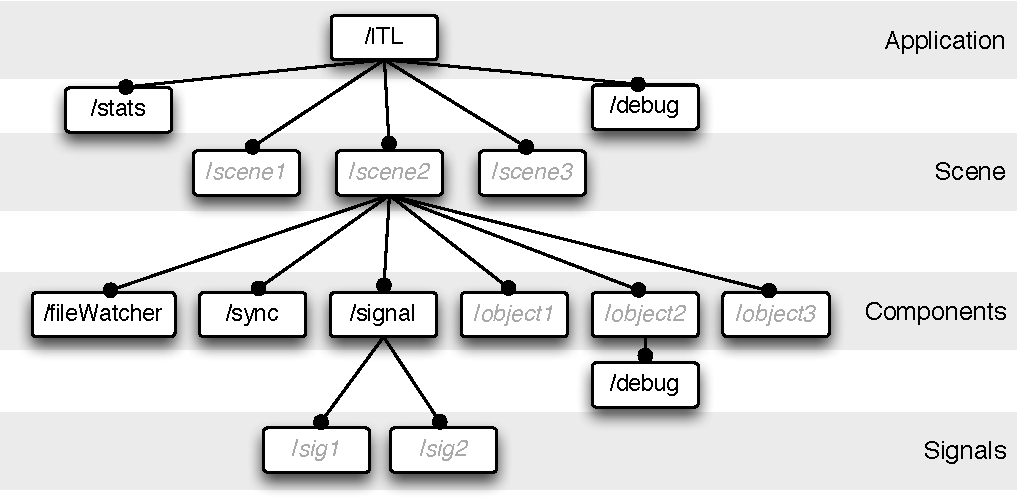
\includegraphics[width=120mm]{imgs/address_space}
 \caption{The OSC address space. Nodes in italic/blue are dynamic nodes.}
 \label{fig:addrspace}
\end{figure}

OSC messages are accepted at any level of the hierarchy:
\begin{itemize}

\item \textbf{the application level} responds to messages for application management (udp ports management, loading files, query messages). \\

\item \textbf{the scene level} contains \emph{scores} that are associated to a window and respond to specific scene management messages. 
It includes a static node named \OSC{stats} that collects information about incoming messages, a static \OSC{log} node that control an embedded log window.


\item \textbf{the component level} contains the score components and 3 static nodes:
\begin{itemize}
\item a \emph{signal} node that may be viewed as a folder containing signals
\item a \emph{sync} node, in charge of the synchronization messages
\item a \emph{javascript} node, that may be adressed to run javascript code dynamically.
\end{itemize}

Each component includes a static node named \OSC{debug} that provides debugging information.
\item \textbf{the signals level} contains signals i.e. objects that accept data streams and that may be graphically rendered as a scene component (see Signals and Graphic signals section \fullref{graphsig}).

\end{itemize}

\note{} Since version 1.05, each component of a score may also be a container and thus, the hierarchy described above has a potential infinite depth level. Note also that a \OSC{sync} node is present at each level. 


%===============================
\sublevel{Aliases}
\label{alias}
An alias mechanism allows an arbitrary OSC address to be used in place of a real address. An \OSC{alias} message is provided to describe aliases: 
\begin{rail}
alias : OSCAddress 'alias' (([1] OSCAlias (message | ) ) | [2])
\end{rail}
\index{Common messages!alias}
\begin{itemize}
\item \textbf{[1]} sets \OSC{OSCAlias} as an alias of \OSC{OSCAddress}. The alias may be optionally followed by a message string which is then taken as an implied message i.e. the alias is translated to \OSC{OSCAddress message}.
\item \textbf{[2]} removes \OSC{OSCAddress} aliases.
\end{itemize}

\example
\sample{/ITL/scene/myobject alias '/1/fader1';}
\sampleindent makes the object \OSC{myobject} addressable using the address \OSC{/1/fader1}.

\note{} Regular expressions are not supported by the alias mechanism and could lead to unpredictable results.



%===============================
%:Common messages
\toplevel{Common messages}
\label{common}
Common messages are intended to control the graphic and the time space of the components of a scene.
They could be sent to any address with the form \OSC{/ITL/\textit{scene}} or \OSC{/ITL/\textit{scene}/\textit{identifier}} where \OSC{\textit{identifier}} is the unique identifier of a scene component.
\begin{rail}
commonMsg :  ('show' int32)
			| 'del'
			| 'export' ([1] ( fullPathFileName) | [2] path | [3])(|'children')
			| 'save' (| 'message' +) filePath ( | '+')
			| PositionMsg
			| ColorMsg
			| TimeMsg
			| WatchMsg
\end{rail}
\index{Common messages!show}
\index{Common messages!del}
\index{Common messages!export}
\index{Common messages!save}

\begin{itemize}
\item \OSC{show}: shows or hides the destination object. The parameter is interpreted as a boolean value. Default value is \values{1}. 
\item \OSC{del}: deletes the destination object. 

\item \OSC{export}: exports an object to an image file. \\
1) exports to a full path name. The file extension is used to infer the export format. Supported extensions and formats are: \emph{pdf, bmp, gif, jpeg, png, pgm, ppm, tiff, xbm, xpm}. \\
2) exports to \OSC{path/\textit{identifier}.pdf}. \\
When path is a relative path, exports to \OSC{rootPath/path/\textit{identifier}.pdf}. \\
3) exports to \OSC{rootPath/\textit{identifier}.pdf}.\\
When the destination file is not completely specified (third form or missing extension), there is an automatic numbering of output names when the destination file already exists. \\ 
The 'children' option specify that we want to export the children of the object as well.

\item \OSC{save}: recursively saves objects states to a file. When a \OSC{message} list is present, only the specified attributes are saved. The \OSC{filePath} can be relative or absolute. When relative, an absolute path is build using the current \OSC{rootPath} (see application or scene current paths  p.\pageref{applmgmt} and  p.\pageref{scene}). The optional \OSC{+} parameter indicates an append mode for the write operation. The message must be sent to the address \OSC{/ITL} to save the whole application state.\\
\textbf{Note}: when a list of attributes is specified, unknown attributes are silently ignored. \\
\textbf{Note}: the file extension for INScore files is \OSC{.inscore}. INScore files dropped on the application or on a window are interpreted as script files (see section \fullref{scripting}).

%\item \OSC{rename}: rename the destination object. Changes its OSC address. \textbf{Warning}: OSC pattern matching allows to give the same name to a whole collection of objects; in this case, there is no way to individually address an object when its name is shared with other objects.
\item 'PositionMsg' are absolute and relative position messages.
\item 'ColorMsg' are absolute and relative color control messages.
\item 'TimeMsg' are time management messages. They are described in section \fullref{time}.
\item 'WatchMsg' are described in section \fullref{interaction}.
%\item 'clickSelectMsg' are provided to query objects relative positions.
\end{itemize}

\example \\
Export of a scene to a given file as jpeg at the current root path:
\sample{/ITL/scene export 'myexport.jpg';}
Saving a scene to \OSC{myScore.inscore} at the current root path, the second form saves only the \OSC{x}, \OSC{y} and \OSC{z} attributes, the third form uses the append mode:
\sample{/ITL/scene save 'myScore.inscore';\\
/ITL/scene save x y z 'thePositions.inscore'; \\
/ITL/scene save 'myScore.inscore' '+';}
Hiding an object:
\sample{/ITL/scene/myObject show 0;}

%-------------------------------
%:    Positioning
\sublevel{Positioning}

\begin{rail}
PositionMsg : 		absPosMsg 
				|	relPosMsg 
				|	originMsg 
				| 	transformMsg
\end{rail}

Graphic position messages are absolute position or relative position messages. They can also control an object \emph{origin} and transformations like rotation around an axis.

\subsublevel{Absolute positioning}

\begin{rail}
absPosMsg :  
			('x' float32)
		| 	('y' float32)
		| 	('z' float32)
		| 	('angle' float32)
		| 	('scale' float32) 
\end{rail}
\index{Position messages!absolute!x}
\index{Position messages!absolute!y}
\index{Position messages!absolute!z}
\index{Position messages!absolute!angle}
\index{Position messages!absolute!scale}
\index{Common messages!x}
\index{Common messages!y}
\index{Common messages!z}
\index{Common messages!angle}
\index{Common messages!scale}

\begin{itemize}
\item \OSC{x y}: moves the \values{x} or \values{y} coordinate of a component. By default, components are centered on their \values{x}, \values{y} coordinates. The coordinates space range is \values{[-1,1]}. \\
For a \OSC{scene} component, -1 is the leftmost or topmost position, 1 is the rightmost or bottommost position. \values{[0,0]} represents the center of the \OSC{scene}. \\
For the \OSC{scene} itself, it moves the window in the screen space and the coordinate space is orthonormal, based on the screen lowest dimension (\emph{i.e.} with a 4:3 screen, \OSC{y=-1} and \OSC{y=1} are respectively the exact top and bottom of the screen, but neither \OSC{x=-1} nor \OSC{x=1} are the exact left and right of the screen). \\
Default coordinates are \values{[0,0]}.
\item \OSC{z}: sets the \values{z} order of a component. \values{z} order is actually relative to the \OSC{scene} components: objects of high \values{z} order will be drawn on top of components with a lower \values{z} order. Components sharing the same \values{z} order will be drawn in an undefined order, although the order will stay the same for as long as they live. \\
Default \values{z} order is 0.
\item \OSC{angle}: sets the \values{angle} value of a component, which is used to rotate it around its center. The angle is measured in clockwise degrees from the \values{x} axis.\\
Default angle value is 0.
\item \OSC{scale}: reduce/enlarge a component. Default scale is \values{1}.
\end{itemize}

\example \\
Moving and scaling an object:
\sample{/ITL/scene/myObject x -0.9; \\
/ITL/scene/myObject y 0.9; \\
/ITL/scene/myObject scale 2.0;
}

%-------------------------------
%:    Relative positioning
\subsublevel{Relative positioning}
\label{relpos}

\begin{rail}
relPosMsg :  
			('dx' float32)
		| 	('dy' float32)
		| 	('dz' float32)
		| 	('drotatex' float32)
		| 	('drotatey' float32)
		| 	('drotatez' float32)
		| 	('dangle' float32)
		| 	('dscale' float32) 
\end{rail}
\index{Position messages!relative!dx}
\index{Position messages!relative!dy}
\index{Position messages!relative!dz}
\index{Position messages!relative!dangle}
\index{Position messages!relative!drotatex}
\index{Position messages!relative!drotatey}
\index{Position messages!relative!drotatez}
\index{Position messages!relative!dscale}
\index{Common messages!dx}
\index{Common messages!dy}
\index{Common messages!dz}

\begin{itemize}
\item \OSC{dx}, \OSC{dy}, \OSC{dz} messages are similar to \OSC{x}, \OSC{y}, \OSC{z} but the parameters represent a displacement relative to the current target value.
\item \OSC{drotatex}, \OSC{drotatey}, \OSC{drotatez} are relative rotation messages. \OSC{dangle} is equivalent to \OSC{drotatez} and is maintained only for compatibility reasons.
\item \OSC{dscale} is similar to \OSC{scale} but the parameters represents a scale multiplying factor.
\end{itemize}

\example \\
Relative displacement of an object:
\sample{/ITL/scene/myObject dx 0.1;}

%-------------------------------
%:    Components origin
\subsublevel{Components origin}
\label{origin}

The origin of a component is the point \values{(xo, yo)} such that the \values{(x, y)} coordinates and the \values{(xo, yo)} point coincide graphically. For example, when the origin is the top left corner, the component top left corner is drawn  at the \values{(x, y)} coordinates.

\begin{rail}
originMsg :  
			('xorigin' float32)
		| 	('yorigin' float32)
		| 	('dxorigin' float32)
		| 	('dyorigin' float32)
\end{rail}
\index{Position messages!relative!xorigin}
\index{Position messages!relative!yorigin}
\index{Position messages!relative!dxorigin}
\index{Position messages!relative!dyorigin}

\begin{itemize}
\item \OSC{xorigin}, \OSC{yorigin} are relative to the component coordinates space i.e. \values{[-1,1]}, where -1 is the top or left border and 1 is the bottom or right border. The default origin is \values{[0,0]} i.e. the component is centered on its \values{(x,y)} coordinates.
\item \OSC{dxorigin}, \OSC{dyorigin} represents displacement of the current \OSC{xorigin} or \OSC{yorigin}.
\end{itemize}

\example \\
Setting an object graphic origin to the top left corner.
\sample{/ITL/scene/myObject xorigin -1. ;\\
/ITL/scene/myObject yorigin -1. ;
}

%-------------------------------
%:    Components transformations
\sublevel{Components transformations}
\label{transform}

A component tranformation specifies 2D transformations of its coordinate system. It includes shear and object rotation.

\begin{rail}
transformMsg :
			(('rotatex' | 'rotatey' | 'rotatez') float32)
		| 	('shear' x y)
\end{rail}
\index{Transform messages!rotate}
\index{Transform messages!shear}

\begin{itemize}
\item \OSC{rotatex rotatey rotatez}: rotates the component around the corresponding axis. Parameter value expresses the rotation in degrees.
\item \OSC{shear} transforms the component in x and y dimensions. \OSC{x} and \OSC{y} are float values expressing the transformation value in the corresponding dimension.
\end{itemize}

\example \\
Rotating an object graphic on the \OSC{z} axis.
\sample{/ITL/scene/myObject rotatez 90. ;}

\note{} \OSC{angle} and \OSC{rotatez} are equivalent. \OSC{angle} has been introduced before the transformation messages and is maintained for compatibility reasons.

%-------------------------------
%:Color messages
\sublevel{Color messages}
\label{colormsg}


\begin{rail}
ColorMsg : 	absColorMsg 
			|	relColorMsg 
\end{rail}

Color messages are absolute or relative color control messages. Color may be expressed in RGBA or HSBA.

\subsublevel{Absolute color messages}

\begin{rail}
absColorMsg :    color
			| hsb
			| 'red' colorvalue
			| 'green' colorvalue
			| 'blue' colorvalue
			| 'alpha' colorvalue
			| 'hue' colorvalue
			| 'saturation' colorvalue
			| 'brightness' colorvalue
\end{rail}
\index{Common messages!color}
\index{Common messages!color!red}
\index{Common messages!color!blue}
\index{Common messages!color!green}
\index{Common messages!color!alpha}
\index{Common messages!color!hue}
\index{Common messages!color!saturation}
\index{Common messages!color!brightness}


\OSC{red}, \OSC{green}, \OSC{blue}, \OSC{hue}, \OSC{saturation}, \OSC{brightness}, \OSC{alpha} messages address a specific part of a color using the RGB or HSB scheme.

\begin{rail}
colorvalue :    int32 | float32
\end{rail}

The value may be specified as integer or float. The data range is given in table \ref{colorrange}.
When the alpha component is not specified, the color is assumed to be opaque. 

\begin{table}[htdp]
\begin{center}
\begin{tabular}{|r|c|c|}
\hline
Component & integer range & float range \\
\hline
\OSC{red} [R] 		& [0,255] & [-1,1] \\
\OSC{green} [G] 	& [0,255] & [-1,1] \\
\OSC{blue} [B]		& [0,255] & [-1,1] \\
\OSC{alpha} [A] 	& [0,255] & [-1,1] \\
\OSC{hue} [H] 		& [0,360] & [-1,1] mapped to [-180,180]\\
\OSC{saturation} [S] 	& [0,100] & [-1,1] \\
\OSC{brightness} [B] 	& [0,100] & [-1,1] \\
\hline
\end{tabular}
\end{center}
\caption{Color components data ranges when expressed as integer or float.}
\label{colorrange}
\end{table}%


\example \\
The same alpha channel specified as integer value or as floating point value:
\sample{/ITL/scene/myObject alpha 51 ;\\
/ITL/scene/myObject alpha 0.2 ;
}

\subsublevel{The color messages}

\begin{rail}
color :		'color' ('r' 'g' 'b' | 'r' 'g' 'b' 'a') 
\end{rail}
\index{Common messages!color}

\OSC{color} sets an object color in the RGBA space.
When A is not specified, the color is assumed to be opaque. 
Default color value is \values{[0,0,0,255]}.


\subsublevel{The hsb messages}

\begin{rail}
hsb :		'hsb' ('h' 's' 'b' | 'h' 's' 'b' 'a') 
\end{rail}
\index{Common messages!hsb}

\OSC{hsb} sets an object color in the HSBA space. 
When A is not specified, the color is assumed to be opaque. 



%-------------------------------
%:    Relative color messages
\subsublevel{Relative color messages}
\label{relcolormsg}

\begin{rail}
relColorMsg :  
		 	('dcolor' color) 
		| 	('dhsb' hsb) 
		| 	('dred' colorvalue) 
		| 	('dgreen' colorvalue) 
		| 	('dblue' colorvalue) 
		| 	('dhue' colorvalue) 
		| 	('dsaturation' colorvalue) 
		| 	('dbrightness' colorvalue) 
		| 	('dalpha' colorvalue) 
\end{rail}
\index{Position messages!color!dcolor}
\index{Position messages!color!dhsb}
\index{Position messages!color!dred}
\index{Position messages!color!dgreen}
\index{Position messages!color!dblue}
\index{Position messages!color!dhue}
\index{Position messages!color!dsaturation}
\index{Position messages!color!dbrightness}
\index{Position messages!color!dalpha}

\begin{itemize}
\item \OSC{dred}, \OSC{dgreen}, etc. messages are similar to \OSC{red}, \OSC{green}, etc. messages but the parameters values represent a displacement of the current target value.
\item \OSC{dcolor} and \OSC{dhsb} are similar and each color parameter represents a displacement of the corresponding target value.
\end{itemize}

\example \\
Moving a color in the RGBA space:
\sample{TL/scene/myObject dcolor 10 5 0 -10 ,}
\sampleindent will increase the red component by 10, the blue component by 5, and decrease the transparency by 10.

\note{} Objects that are carrying color information (images, SVG) don't respond to color change but are sensitive to transparency changes.


%-------------------------------
%:'effect' messages
\sublevel{The 'effect' messages}
\label{effectmsg}

The \OSC{effect} message sets a graphic effect on the target object.

\begin{rail}
effectMsg : 'effect' ( 'none'
		| ('blur'
		| 'colorize'
		| 'shadow') (| params)) 		
\end{rail}
\index{Effect messages!effect!none}
\index{Effect messages!effect!blur}
\index{Effect messages!effect!colorize}
\index{Effect messages!effect!shadow}

\begin{itemize}
\item \OSC{none}: removes any effect set on the target object.
\item \OSC{blur, colorize, shadow}: sets the corresponding effect. An effect always replaces any previous effect. The effect name is followed by optional specific effects parameters.
\end{itemize}

\note{} An effect affects the target object but also all the target slaves.

\subsublevel{The blur effect}

\begin{rail}
blurParams : int32 (| blurHint)
\end{rail}

Blur parameters are the blur radius and a rendering hint. The radius is an int32 value. By default, it is 5 pixels. The radius is given in device coordinates, meaning it is unaffected by scale. 

\begin{rail}
blurHint : 'performance' | 'quality' | 'animation'
\end{rail}
Use the \OSC{performance} hint to say that you want a faster blur, the \OSC{quality} hint to say that you prefer a higher quality blur, or the \OSC{animation} when you want to animate the blur radius. The default hint value is \OSC{performance}.

\example \\
Setting a 8 pixels effect on \OSC{myObject}
\sample{/ITL/scene/myObject effect blur 8;}

\subsublevel{The colorize effect}

\begin{rail}
colorizeParams : float32 (| color)
\end{rail}

Colorize parameters are a strength and a tint color. The strength is a float value. By default, it is 1.0. A strength 0.0 equals to no effect, while 1.0 means full colorization. \\
The color is given as a RGB triplet (see section \fullref{colormsg}) by default, the color value is light blue (0, 0, 192).

\example \\
Setting a red colorize effect on \OSC{myObject} with a 0.5 strength.
\sample{/ITL/scene/myObject effect colorize 0.5 200 0 0;}


\subsublevel{The shadow effect}

\begin{rail}
shadowParams : xoffset yoffset (| color (| blur))
\end{rail}

\OSC{xoffset} and \OSC{yoffset} are the shadow offset and should be given as int32 values. The default value is 8 pixels. The offset is given in device coordinates, which means it is unaffected by scale. \\
The color is given as a RGBA color (see section \fullref{colormsg}) by default, the color value is a semi-transparent dark gray (63, 63, 63, 180) \\
The blur radius should be given as an int32 value. By default, the blur radius is 1 pixel.

\example \\
Setting a shadow effect on \OSC{myObject}. \\
The shadow offset is (10,10) pixels, the color is a transparent grey (100,100,100, 50) and the blur is 8 pixels.
\sample{/ITL/scene/myObject effect shadow 10 10 100 100 100 50 8;}


%===============================
%:Time management messages
\toplevel{Time management messages}
\label{time}
Time messages control the time dimension of the score components. They could be sent to any address with the form \OSC{/ITL/\textit{scene}/\textit{identifier}} where \OSC{\textit{identifier}} is the unique identifier string of a scene component.
\begin{rail}
timeMsg : 'clock'
		| 'durClock' 
		| ('date' time)
		| ('duration' time) 
		| ('ddate' time) 
		| ('dduration' time) 
\end{rail}
\index{Time messages!absolute!date}
\index{Time messages!absolute!duration}
\index{Time messages!relative!ddate}
\index{Time messages!relative!dduration}
\index{Time messages!relative!clock}
\index{Time messages!relative!durClock}

\begin{rail}
time : (([1] int32 int32) | [2] int32 | [3] float32 | [4] 'n/d')
\end{rail}

\begin{itemize}
\item 1) Time is specified as a rational value \values{d/n} where \values{1/1} represents a whole note. 
\item 2) Time may be specified with a single integer, then 1 is used as implicit denominator value.
\item 3) Time may be specified as a single float value that is converted using the following approximation: let \values{f} be the floating point date, the corresponding rational date is computed as \values{f x 10000 / 10000}.
\item 4) Time may also be specified as a string in the form \OSC{'n/d'}.
\end{itemize}

\begin{itemize}
\item \OSC{clock}: similar to MIDI clock message: advances the object date by 1/24 of quarter note.
\item \OSC{durClock}: a clock message applied to duration: increases the object duration by 1/24 of quarter note.
\item \OSC{date}: sets the time position of an object. Default value is \values{0/1}.
\item \OSC{duration}: changes the object duration. Default value is \values{1/1}.
\item \OSC{ddate}: relative time positioning message: adds the specified value to the object date.
\item \OSC{dduration}: relative duration message: adds the specified value to the object duration.
\end{itemize}


\example \\
Various ways to set an object date.
\sample{/ITL/scene/myObject date 2 1 ;\\
/ITL/scene/myObject date 2;     \hspace{1.2cm}// the denominator is 1 (implied) \\
/ITL/scene/myObject date 0.5;   \hspace{7mm} // equivalent to 1/2 \\
/ITL/scene/myObject date '1/2'; \hspace{4mm} // the string form
}
Similar ways to move an object date.
\sample{/ITL/scene/myObject clock;   \\
/ITL/scene/myObject ddate '1/96';
}


%===============================
%:The 'set' message
\toplevel{The 'set' message}
\label{setsect}
The \OSC{set} messages can be sent to any address with the form \OSC{/ITL/scene/\textit{identifier}}. The global form of the message is:

\begin{rail}
setMsg : 'set' type data
\end{rail}

It sets a \OSC{scene} component data. 

When there is no destination for the OSC address, the component is first created before being given the message. 

When the target destination type doesn't correspond to the message \OSC{type}, the object is replaced by an adequate object.

%===============================
%:  Symbolic music notation
\sublevel{Symbolic music notation}
\label{symscore}

Symbolic music notation support is based on the Guido Music Notation format [GMN] or on the MusicXML format. MusicXMl is supported via conversion to the GMN format when the MusicXML library is present.

\begin{rail}
setMsg : 'set' (
	('gmn' gmnString) |
	('gmnf' gmnFilePath) |
	('gmnstream' gmnStream) |
	('musicxml' xmlString) |
	('musicxmlf' xmlFilePath)
)
\end{rail}
\index{Common messages!set}
\index{Set type!gmn}
\index{Set type!gmnf}
\index{Set type!gmnstream}
\index{Set type!musicxml}
\index{Set type!musicxmlf}

\begin{itemize}
\item \OSC{gmn}: a Guido score defined by a GMN string.
\item \OSC{gmnf}: a Guido score defined by a GMN file.
\item \OSC{gmnstream}: a Guido score defined by a GMN stream (a GMN string that can be written in several times).
\item \OSC{musicxml}: a score defined by a MusicXML string.
\item \OSC{musicxmlf}: a score defined by a MusicXML file.
\end{itemize}

\example \\
Creating a music score using a Guido Music Notation language string.
\sample{/ITL/scene/myObject set gmn "[ a b g ]";}
Creating the same music score as a stream.
\sample{/ITL/scene/myObject set gmnstream "[ a";\\
/ITL/scene/myObject write "b";\\
/ITL/scene/myObject write "g";
}

\note{} For compatibility with previous versions, passing a MusicXML string to a \OSC{gmn} object or a MusicXML file to a \OSC{gmnf} object may succed since the system tries to parse the content as GMN content or as MusicXML content when the former fails.

\note{} Conversion from MusicXML to GMN could be achieved manually using a command line tool that is distributed with the MusicXML library (see at \url{http://code.google.com/p/libmusicxml/}). It allows to improve the output GMN code afterhand.

%===============================
%:  Textual components
\sublevel{Textual components}
\label{textscore}

\begin{rail}
setMsg : 'set' (
	('txt' (string | txtStream)) |
	('txtf' textFilePath) |
	('html' string) |
	('htmlf' htmlFilePath)
)
\end{rail}
\index{Set type!txt}
\index{Set type!html}
\index{Set type!txtf}
\index{Set type!htmlf}

\begin{itemize}
\item \OSC{txt}: a textual component.
\item \OSC{txtf}: a textual component defined by a file.
\item \OSC{html}: an html component defined by an HTML string.
\item \OSC{htmlf}: an html component defined by an HTML file.
\end{itemize}

Text may be specified by a single quoted string or using an arbitrary count of parameters that are converted to a single string with a space used as separator.
\begin{rail}
txtStream :  (string | int32 | float32) +
\end{rail}

\example \\
Creating a text object.
\sample{/ITL/scene/myObject set txt "Hello ...    world!";}
Setting the content of a text object using a values stream.
\sample{/ITL/scene/myObject set txt Hello 1 world and 0.5; }


%===============================
%:  Vectorial graphics
\sublevel{Vectorial graphics}
\label{vgraphscore}
\begin{rail}
setMsg : 'set' (
	('svg' svgString) |
	('svgf' svgFilePath) |
	('rect' width height) |
	('ellipse' width height) |
	('polygon' ( (x y) +)) |
	('curve' ((x1 y1 x2 y2 x3 y3 x4 y4) +)) |
	('line' ('xy' x y | 'wa' width angle)) |
)
\end{rail}
\index{Set type!svg}
\index{Set type!svgf}
\index{Set type!rect}
\index{Set type!ellipse}
\index{Set type!polygon}
\index{Set type!curve}
\index{Set type!line}

\begin{itemize}
\item \OSC{svg}: SVG graphics defined by a SVG string.
\item \OSC{svgf}: vectorial graphics defined by a SVG file.
\item \OSC{rect}: a rectangle specified by a width and height. Width and height are expressed in \OSC{scene} coordinates space, thus a width or a height of 2 corresponds to the width or a height of the \OSC{scene}.
\item \OSC{ellipse}: an ellipse specified by a width and height.
\item \OSC{polygon}: a polygon specified by a sequence of points, each point being defined by its (x,y) coordinates. The coordinates are expressed in the \OSC{scene} coordinate space, but only the relative position of the points is taken into account (\emph{i.e} a polygon A = \{ (0,0) ; (1,1) ; (0,1) \} is equivalent to a polygon B = \{ (1,1) ; (2,2) ; (1,2) \}).
\item \OSC{curve}: a sequence of 4-points bezier cubic curve. If the end-point of a curve doesn't match the start-point of the following one, the curves are linked by a straight line. The first curve follows the last curve. The inner space defined by the sequence of curves is filled, using the object color. The points coordinates are handled like in a \OSC{polygon}.
\item \OSC{line}: a simple line specified by a point (x,y) expressed in \OSC{scene} coordinate space or by a width and angle. The point form is used to compute a line from (0,0) to (x,y), which is next drawn centered on the scene.
\end{itemize}

\example \\
Creating a rectangle with a 0.5 width and a 1.5 height.
\sample{/ITL/scene/myObject set rect 0.5 1.5;}
Creating a line specified using width and angle.
\sample{/ITL/scene/myObject set line wa 1. 45.;}


%===============================
%:  Signals and graphic signals
\sublevel{Signals and graphic signals}
\label{sigscore}

Signals are special objects that are stored in a special \OSC{signal} node and that may be composed in parallel to produce graphic signals. Signals and graphic signals are decribed in section \fullref{graphsig}.

Signals and computation on signals may be based on FAUST objects that are actually signals processors. FAUST objects are decribed in section \fullref{faust}. \\
For more information about the FAUST language, see at \url{http://faust.grame.fr}.

\begin{rail}
setMsg : 'set' (
	('graph' signals ) |
	('fastgraph' signals ) |
	('faust' 'pluginname' ) |
	('faustdsp' faustcode ) |
	('faustdspf' faustfile)
)
\end{rail}
\index{Set type!graph}
\index{Set type!fastgraph}
\index{Set type!faust}
\index{Set type!faustdsp}

\begin{itemize}
\item \OSC{graph}: graphic of a signal. See section \fullref{graphsig} for details about the \OSC{graph} objects data.
\item \OSC{fastgraph}: fast rendering graphic signal. See also section \fullref{graphsig}.
\item \OSC{faust}: a FAUST object as a plugin (see section \ref{faust})
\item \OSC{faustdsp}: a FAUST object defined by a string (see section \fullref{faust})
\item \OSC{faustdspf}: a FAUST object defined by a file (see section \fullref{faust})
\end{itemize}


%===============================
%:  Images and video
\sublevel{Images and video}
\label{imgscore}

Images and video are supported using various formats. See section \fullref{fileset} for more details on the supported formats.

\begin{rail}
setMsg : 
	('img' imgPath) |
	('video' videoPath)
\end{rail}
\index{Set type!img}
\index{Set type!video}

\begin{itemize}
\item \OSC{img}: animage file. The image format is infered from the file extension.
\item \OSC{video}: a video file. The video format is infered from the file extension. Note that navigation through the video is made using its \OSC{date}.
\end{itemize}

\example \\
Creating an image.
\sample{/ITL/scene/myObject set img "myImage.png";}


%===============================
%:  Miscellaneous
\sublevel{Miscellaneous}
\label{miscscore}

\begin{rail}
setMsg : 'set' (
	'layer'  |
	('grid' int32 int32)
)
\end{rail}
\index{Set type!layer}
\index{Set type!grid}

\begin{itemize}
\item \OSC{layer}: a graphic layer, may be viewed as a container (see \fullref{layers}).
\item \OSC{grid}: a white transparent object that provides a predefined time to graphic mapping (see section \fullref{grid} for more details and section \fullref{mapping} for time to graphic relations). The parameters are int32 values representing the number of columns and rows.
\end{itemize}


%===============================
%:  The file type
\sublevel{The file type}
\label{fileset}

\label{setfile}
\begin{rail}
setFile : 
	('file' filePath)
\end{rail}
\index{Set type!file}

\begin{itemize}
\item \OSC{file}: a generic type to handle file based objects. Actually, the \OSC{file} type is translated into a one of the \OSC{txtf}, \OSC{gmnf}, \OSC{img} or \OSC{video} types, according to the file extension (see table \ref{fileTranslate}).
\end{itemize}

\seealso the application \OSC{rootPath} message (section \fullref{ITL}) for file based objects.

\begin{table}[htdp]
\caption{File extensions supported by the \OSC{file} translation scheme.}
\begin{center}
\begin{tabular}{|r|c|}
\hline
file extension & translated type \\
\hline
\OSC{.txt .text}		& \OSC{txtf} \\
\OSC{.htm .html}		& \OSC{htmlf} \\
\OSC{.gmn}			& \OSC{gmnf} \\
\OSC{.xml}			& \OSC{musicxmlf} \\
\OSC{.svg} 			& \OSC{svgf} \\
\OSC{.jpg .jpeg .png .gif .bmp .tiff} & \OSC{img} \\
\OSC{.avi .wmv .mpg .mpeg .mp4 .mov .vob} & \OSC{video} \\
\OSC{.dsp} 			& \OSC{faustdspf} \\
\hline
\end{tabular}
\end{center}
\label{fileTranslate}
\end{table}

\example \\
Creating an image using the \OSC{file} type.
\sample{/ITL/scene/myObject set file "myImage.png"; \\
will be translated into \\
/ITL/scene/myObject set img "myImage.png";
}


%===============================
%:The 'get' message
\toplevel{The 'get' messages}
\label{getsect}

%-------------------------------
%\sublevel{Common 'get' format}
The \OSC{get} messages can be sent to any valid OSC address. It is intended to query the system state. It is the counterpart of all the messages modifying this state.  The result of the query is sent to the OSC output port with the exact syntax of the counterpart message. 
The global form of the message is:
\begin{rail}
getMsg : 'get' ( | getParam +)
\end{rail}
\index{Common messages!get}

The \OSC{get} message without parameter is the counterpart of the \OSC{set} message. When addressed to a container (the application \OSC{/ITL}, a scene \OSC{/ITL/scene}, the signal node \OSC{/ITL/scene/signal}) is also distributed to all the container components.

Specific \OSC{get} forms may be available, depending on the component type (see sections \ref{gmnpage},  \ref{ITLQuery}, \ref{ITLdebug}, \ref{syncmsg}, \ref{parcomp}, \ref{faustmsg}).

\example \\
Sending the following request to an object which position is 0.3 0.5
\sample{/ITL/scene/myobject get x y;}
\sampleindent will give the following messages on outpout port:
\sample{/ITL/scene/myobject x 0.3; \\
/ITL/scene/myobject y 0.5;}
Querying an object content
\sample{/ITL/scene/myobject get;}
\sampleindent will give the corresponding \OSC{set} message:
\sample{/ITL/scene/myobject set txt "Hello world!";}

\note{} \\
The \OSC{get width} and \OSC{get height} messages addressed to components that have no explicit width and height (text, images, etc.) returns 0 as long as the target component has not been drew.



%===============================
%:Type specific messages
\toplevel{Type specific messages}
\label{specificMsg}
Some of the messages are specific to the component \OSC{type}.


%-------------------------------
\sublevel{Pen control}

Specific pen messages accepted by the components types \OSC{rect | ellipse | polygon | curve | line | graph | fast graph | grid}.
\begin{rail}
penMsg : 	  'penColor' color 
			| 'penAlpha' colorvalue
			| 'pendAlpha' colorvalue
			| 'penWidth' float32
			| 'penStyle' penstyle
\end{rail}
\index{Specific messages! penColor}
\index{Specific messages! penAlpha}
\index{Specific messages! pendAlpha}
\index{Specific messages! penWidth}
\index{Specific messages! penStyle}

\begin{itemize}
\item \OSC{penColor} controls the pen color. The color should be given in the RGBA space. The default value is opaque black (0 0 0 255).
\item \OSC{penAlpha, pendAlpha} controls the pen transparency only. See section \fullref{colormsg} for the expected \item \OSC{penWidth} controls the pen width. The default value is 0 (excepted for \OSC{line} objects, where 1.0 is the default value). It is expressed in arbitrary units (1 is a reasonable value).
\item \OSC{penStyle} controls the pen style.
 \end{itemize}


\begin{rail}
penstyle : 'solid' | 'dash' | 'dot' | 'dashDot' | 'dashDotDot'
\end{rail}
\index{Specific messages! penStyle! solid}
\index{Specific messages! penStyle! dash}
\index{Specific messages! penStyle! dot}
\index{Specific messages! penStyle! dashDot}
\index{Specific messages! penStyle! dashDotDot}

The pen style default value is \OSC{solid}.\\

\example \\
Setting a rectangle border width and color:
\sample{/ITL/scene/rect set rect 0.5 0.5 ;\\
/ITL/scene/rect penWidth 2. ;\\
/ITL/scene/rect penColor 255 0 0 ;  
}


%-------------------------------
\sublevel{Brush control}
\label{brush}
Specific brush messages accepted by the components types \OSC{rect | ellipse | polygon | curve |  layer}.
\begin{rail}
brushMsg : 	  'brushStyle' ('solid' | 'dense1' | 'dense2' | 'dense3' | 'dense4' | 'dense5' | 'dense6' | 'dense7' | 'none' | 'hor' | 'ver' | 'cross' | 'bdiag' | 'fdiag' | 'diagCross')
\end{rail}
\index{Specific messages! brushColor}

\begin{itemize}
\item \OSC{brushStyle} controls the brush style.
 \end{itemize}

\index{Specific messages! brushStyle! solid}
\index{Specific messages! brushStyle! dense}
\index{Specific messages! brushStyle! dense2}
\index{Specific messages! brushStyle! dense3}
\index{Specific messages! brushStyle! dense4}
\index{Specific messages! brushStyle! dense5}
\index{Specific messages! brushStyle! dense6}
\index{Specific messages! brushStyle! dense7}
\index{Specific messages! brushStyle! none}
\index{Specific messages! brushStyle! hor}
\index{Specific messages! brushStyle! ver}
\index{Specific messages! brushStyle! cross}
\index{Specific messages! brushStyle! bdiag}
\index{Specific messages! brushStyle! fdiag}
\index{Specific messages! brushStyle! diagCross}
\index{Specific messages! brushStyle! linearCross}

The brush style default value is \OSC{solid}.\\
For the \OSC{layer} object, the brush style default value is \OSC{none}.\\

\example \\
Setting a rectangle style :
\sample{/ITL/scene/rect set rect 0.5 0.5 ;\\
/ITL/scene/rect brushStyle dense4; 
}


%-------------------------------
\sublevel{Width and height control}

Specific width and height messages accepted by the components types \OSC{rect | ellipse | graph | fastgraph | grid}.

\begin{rail}
widthMsg :  'width' float32
			| 'height' float32
\end{rail}
\index{Specific messages! width}
\index{Specific messages! height}



%-------------------------------
\sublevel{Symbolic score management}
\label{gmnpage}

Messages accepted by the components types \OSC{gmn | gmnstream | gmnf}. 
\begin{rail}
scoreMsg :      'page' int32
			| 'dpage' int32
			| 'pageFormat' float32 float32
			| 'columns' int32
			| 'rows' int32
			| 'get' ( 'pageCount'| 'systemCount' )
\end{rail}
\index{Specific messages! score! page}
\index{Specific messages! score! dpage}
\index{Specific messages! score! pageFormat}
\index{Specific messages! score! columns}
\index{Specific messages! score! rows}
\index{Specific messages! score! pageCount}
\index{Specific messages! score! systemCount}


\begin{itemize}
\item \OSC{page}: set the score current page
\item \OSC{dpage}: moves the score current page
\item \OSC{pageFormat}: set the page format. The parameters are the page width and height. Note that the message has no effect when the score already includes a \verb+\+pageformat tag.
\item \OSC{columns}: for multi pages display: set the number of columns.
\item \OSC{rows}: for multi pages display: set the number of rows.
\item \OSC{pageCount}:  a read only attribute, gives the score pages count.
\item \OSC{systemCount}:  a read only attribute, gives the number of systems on each of the score pages. The result is given as a list systems count ordered by page number (index 0 is page 1, etc.).
\end{itemize}


\example \\
Displaying a multi-pages score on two pages starting at page 3:
\sample{/ITL/scene/myScore columns 2 ;\\
/ITL/scene/myScore page 3 ;
}


\begin{rail}
gmnstreamMsg :      'write' gmnStream
				| 'clear' 
\end{rail}
\index{Specific messages! score! write}
\index{Specific messages! score! clear}

\begin{itemize}
\item \OSC{write}: add the stream in parameter to the global stream
\item \OSC{clear}: reinitialize the stream
\end{itemize}


\example \\
Writing a score in 3 steps:
\sample{/ITL/scene/myScore set gmnstream "[ c"; \\
/ITL/scene/myScore write " d e";\\
/ITL/scene/myScore write " f]";
}


%-------------------------------
\sublevel{The 'grid' object}
\label{grid}

The \OSC{grid} object provides a pre-defined time to graphic mapping organized in columns and row. By default, it is not visible (white, transparent) but supports all the attributes of rectangles (color, pen, effects, etc.). Each element of a grid has a duration that is computed as the grid duration divided by the total number of elements ( columns x rows) and is placed in the time space from the date 0 to the end of the grid duration.

\begin{rail}
gridMsg : 'columns' int32
		| ('rows' int32) 
		| ('xborder' float)
		| ('yborder' float)
		| ('order' ('leftright' | 'topbottom'))
\end{rail}

\begin{itemize}
\item \OSC{columns} set the number of columns of the grid,
\item \OSC{rows} set the number of rows of the grid,
\item \OSC{xborder} set the horizontal spacing between the elements of the grid (default is 0.),
\item \OSC{yborder} set the vertical spacing between the elements of the grid (default is 0.),
\item \OSC{order} defines the time order of the elements. By default, elements are organized from left to right first and from top to bottom next (\OSC{leftright}). The \OSC{topbottom} parameter changes this order from top to bottom first and from left to right next.
\end{itemize}

\example \\
Creating a 10 x 10 grid organized from top to bottom with a border:
\sample{/ITL/scene/grid set grid 10 10 ;\\
/ITL/scene/grid xborder 3. ;\\
/ITL/scene/grid yborder 3. ;\\
/ITL/scene/grid order topbottom ;
}


%-------------------------------
\sublevel{The 'layer' object}
\label{layer}

The \OSC{layer} object provides a container of rectangular shape that is not drawn but creates a node to distinguish a group of objects from the rest. It can however be drawn by using the brush control (default brushStyle is 'none').


%===============================
%:  The debug nodes
\sublevel{The 'debug' nodes}
\label{debugnode}

Each component includes a static \OSC{debug} nodes provided to give information about components.
\begin{rail}
debugMsg : 'map' int32
		| ('name' int32) 
\end{rail}
\index{Common messages!debug!map}
\index{Common messages!debug!name}

\begin{itemize}
\item \OSC{map} is used to display the time to graphic mapping. The parameter is a boolean value. Default is 0.
\item \OSC{name} is used to display both the object name and bounding box. The parameter is a boolean value. Default is 0.
\end{itemize}


%===============================
%:Application messages
\toplevel{Application messages}
\label{ITL}
Application messages are accepted by the static OSC address \OSC{/ITL}. 


%===============================
%:  Application management
\sublevel{Application management}
\label{applmgmt}

\begin{rail}
ITLMsg : 'quit' 
		| ('rootPath' path) 
		| ('mouse' ('show' | 'hide'))
		| ('defaultShow' int32)
		| ('load' filePath)
		| ('read' buffer)
		| ('require' float oscMsg)
		| ('time' int32)
		| ('ticks' int32)
		| ('rate' int32)
		| 'hello'
\end{rail}
\index{ITL messages!rootPath}
\index{ITL messages!mouse}
\index{ITL messages!defaultShow}
\index{ITL messages!load}
\index{ITL messages!read}
\index{ITL messages!hello}
\index{ITL messages!require}
\index{ITL messages!rate}
\index{ITL messages!time}
\index{ITL messages!ticks}

\begin{itemize}
\item \OSC{quit}: requests the client application to quit.

\item \OSC{rootPath}: \emph{rootPath} of an Interlude application is the default path where the application reads or writes a file when a relative path is used for this file. The default value is the user home directory. Sending the \OSC{rootPath} message without parameter resets the application path to its default value.

\item \OSC{mouse}: hide or show the mouse pointer.

\item \OSC{defaultShow}: changes the default \OSC{show} status for new objects. \\
The default \OSC{defaultShow} value is 1.

\item \OSC{load}: loads a file previously saved using the \OSC{save} message (see section \fullref{common}). Note that the load operation appends the new objects to the existing scene. When necessary, it is the sender responsibility to clear the scene before loading a file.

\item \OSC{read}: read a buffer that is expected to contain a valid inscore script.

\item \OSC{require}: check that the current INScore version number is equal or greater to the number given as argument. The version number is given as a float value. A message is associated to the \OSC{require} message, which is triggered when the check fails. See section \fullref{interaction} for more details.

\item \OSC{rate}: changes the time task rate. Note that null values are ignored.\\
The default \OSC{rate} value is 10.

\item \OSC{time}: sets the application current time. The time is expressed in milliseconds.

\item \OSC{ticks}: sets the application current ticks count. The ticks count indicates the number of time tasks performed by the application.

\item \OSC{hello}: query the host IP number. The message is intended for ITL applications discovery. Answer to the query has the following format: \\
\oldexample \OSC{IP  inPort outPort errPort} where \OSC{IP} is sent as a string and port numbers as integer values.

\end{itemize}

\example \\
when sending the message:
\sample{/ITL hello;}
\sampleindent the application will answer with the following message:
\sample{/ITL 192.168.0.5  7000 7001 7003}
\sampleindent when it runs on a host which IP number is \OSC{192.168.0.5} using the default port numbers.

%===============================
%:  Ports management
\sublevel{Ports management}
\label{ITLPorts}

\begin{rail}
ITLPortsMsg : ('port' int32)
		| ('outport' int32)
		| ('errport' int32)
\end{rail}
\index{ITL messages!port}
\index{ITL messages!outport}
\index{ITL messages!errport}

Changes the UDP port numbers:
\begin{itemize}
\item \OSC{port} defines the listening port number, 
\item \OSC{outport} defines the port used to send replies to queries, 
\item \OSC{errport} defines the port used to send error messages. 
\end{itemize}
The \OSC{int32} parameter should be a positive value in the range \values{[1024-49150]}. \\
The default \OSC{port}, \OSC{outport} and \OSC{errport} values are 7000, 7001 and 7002.

\note{} \\
Error messages are sent as a single string.

%===============================
%:  Messages forwarding
\sublevel{Messages forwarding}
\label{ITLForward}

The messages handled by the application can be forwarded to arbitrary remote hosts using the \OSC{forward} message. The \OSC{forward} message itself can't be forwarded. 
 
\begin{rail}
ITLMsgForward : ('forward' ( [1] | [2] hostname +))
\end{rail}
\index{ITL messages!forward}

\begin{itemize}

\item 1) removes the set of forwarded destinations,
\item 2) set a list of remote hosts for forwarding. Note that \OSC{hostname} can be any legal host name or IP number, optionally extended with a port number separated by a semi-colon. By default, when no port number is specified, the current application listening port number is used.
\end{itemize}
\example\\
Forwarding messages to \OSC{host1.adomain.org} using the current application listening port number
and to \OSC{host2.adomain.org} on port number 5100.

\sample{/ITL forward host1.adomain.org host2.adomain.org:5100;}

\warning{forwarding messages to the application host results in an infinite loop with unpredictable results. Thus it is not recommended to use the local network broadcast address for forwarding unless using a different UDP port number.}



%===============================
%:  Application level queries
\sublevel{Application level queries}
\label{ITLQuery}

The application supports the \OSC{get} messages for its parameters (see section \fullref{getsect}). In addition, it provides the following messages to query version numbers.

\begin{rail}
ITLRequest : 'get'  ('version' | 'guido-version' | 'musicxml-version')
\end{rail}
\index{ITL messages!version}
\index{ITL messages!guido-version}
\index{ITL messages!musicxml-version}

\begin{itemize}
\item \OSC{version}: version number request.
\item \OSC{guido-version}: Guido engine version number request.
\item \OSC{musicxml-version}: MusicXML and Guido converter version numbers request. Returns "not available" when the library is not found.

\end{itemize}

\example \\
Querying INScore version:
\sample{/ITL get version;}
\sampleindent will give the following as output:
\sample{/ITL version 1.00}

%===============================
%:  Application static nodes
\sublevel{Application static nodes}
\label{ITLStatic}

The application level provides the static nodes - \OSC{stats}, \OSC{debug} and \OSC{log}, available at \OSC{/ITL/stats} \OSC{/ITL/debug} and \OSC{/ITL/log}  to help debugging communication and INScore scripts design.

\subsublevel{The 'stats' nodes}
\label{ITLstat}

\begin{rail}
ITLStats : 'get'  | 'reset'
\end{rail}
\index{ITL stat!get}
\index{ITL stat!reset}

\begin{itemize}
\item \OSC{get} gives the count of handled messages at OSC and UDP levels: the UDP count indicates the count of messages received from the network, the OSC count includes the UDP count and the messages received internally.
\item \OSC{reset} resets the counters to zero. Note that querying the \OSC{stats} node increments at least the OSC the counter.
\end{itemize}

\example \\
Answer to a \OSC{get} message addressed to \OSC{/ITL/stats}
\sample{/ITL/stats osc 15 udp 10}


\subsublevel{The 'debug' nodes}
\label{ITLdebug}

The \OSC{debug} node is used to activate debugging information.
\begin{rail}
ITLdebug : 'osc' int23
\end{rail}
\index{ITL debug!osc}

\begin{itemize}
\item switch the debug mode ON or OFF. The parameter is interpreted as a boolean value. When in debug mode, INScore sends verbose messages to the OSC error port for every message that can't be correctly handled. Debugging is ON by default.
\end{itemize}

\example \\
Error messages generated on error port in debug mode:
\sample{error:  incorrect OSC address: /ITL/stat\\
error:  incorrect parameters: /ITL/scene/foo unknown 0.1\\
error:  incorrect parameters: /ITL/scene/foo x "incorrectType"
}


\subsublevel{The 'log' nodes}
\label{ITLlog}

The \OSC{log} node controls a console window that display all the messages sent to the OSC error port. Typical content is given by the example above.

\begin{rail}
ITLLog : 'show'  int32
		| 'clear'
		| 'wrap' int32
		| 'write' (arg +)
		| 'save' string
\end{rail}
\index{ITL log!show}
\index{ITL log!clear}
\index{ITL log!wrap}
\index{ITL log!save}

\begin{itemize}
\item \OSC{show} show or hides the console. The parameter is a boolean value.
\item \OSC{clear} clear the console window.
\item \OSC{wrap} control line wrapping of the console. The parameter is a boolean value.
\item \OSC{write} write the \OSC{arg} list formatted as a string to the log window.
\item \OSC{save} save the current log content to a file. The parameter is a file name. When expressed as a relative path, the file is saved under the current application root path.
\end{itemize}



\subsublevel{The 'plugins' nodes}
\label{ITLplugins}

The \OSC{plugins} node controls the search path for plugins. See section \fullref{plugins} for more information on plugins and search strategies.

\begin{rail}
ITLPlugin : 'path'  folder
		| 'reset'
\end{rail}
\index{ITL plugin!path}
\index{ITL plugin!reset}

\begin{itemize}
\item \OSC{path} add \OSC{folder} as a user path. The system will look for plugins in this folder first.
\item \OSC{reset} clear the current user path.
\end{itemize}


%===============================
%:Scene messages
\toplevel{Scene messages}
\label{scene}
A scene may be viewed as a window on the score elements. Its address is \OSC{/ITL/\textit{sceneIdentifier}} where \OSC{\textit{sceneIdentifier}} is the scene name. It handles the following messages:
\begin{rail}
sceneMsg :  'new'
			| 'del'
			| 'reset'
			| ('rootPath' path) 
			| ('load' filePath)
			| ('fullscreen' int32)
			| ('frameless' int32)
			| ('absolutexy' int32)
			| ('windowOpacity' int32)
			| commonMsg
\end{rail}
\index{Scene messages}
\index{Scene messages!new}
\index{Scene messages!del}
\index{Scene messages!rootPath}
\index{Scene messages!load}
\index{Scene messages!reset}
\index{Scene messages!fullscreen}
\index{Scene messages!frameless}
\index{Scene messages!absolutexy}

\begin{itemize}
\item \OSC{new}: creates a new scene and opens it in a new window.
\item \OSC{del}: deletes a scene and closes the corresponding window.
\item \OSC{reset}: clears the scene (i.e. delete all components) and resets the scene to its default state (position, size and color).
\item \OSC{rootPath}: \emph{rootPath} of a scene is the default path where the scene reads or writes a file when a relative path is used for this file. When no value has been specified, the application  \emph{rootPath} is used.
\item \OSC{load}: loads an INScore file to the scene. Note that the OSC addresses are translated to the scene OSC address.
%\item \OSC{foreground}: put the scene to foreground.
\item \OSC{fullscreen}: requests the scene to switch to full screen or normal screen.  The parameter is interpreted as a boolean value. Default value is \values{0}.
\item \OSC{frameless}: requests the scene to switch to frameless or normal window.  The parameter is interpreted as a boolean value. Default value is \values{0}.
\item \OSC{absolutexy}: requests the scene to absolute or relative coordinates. Absolute coordinates are in pixels relative to the top left corner of the screen. Relative coordinates are in the range [-1, 1] where [0,0] is the center of the screen. The message parameter is interpreted as a boolean value. Default value is \values{0}.
\item \OSC{windowOpacity}: switch the scene window to opaque or transparent mode. When in transparent mode, the scene alpha channel controls the window opacity (from completely opaque to completely transparent). In opaque mode, the scene alpha channel controls the background brush only. Default value is \values{0}.
\item \OSC{commonMsg}: a scene support the common graphic attributes. See section \fullref{common}.
\end{itemize}

\example \\
Setting a scene current path:
\sample{/ITL/scene rootPath "/path/to/my/folder";}
Loading an INScore file:
\sample{/ITL/scene load "myscript.inscore";}
\sampleindent will load \OSC{/path/to/my/folder/myscript.inscore} into the scene. 

Setting a scene to fullscreen:
\sample{/ITL/scene fullscreen 1;}
Creating a new score named \OSC{myScore}:
\sample{/ITL/myScore new;}


%===============================
%:Layers
\toplevel{Layers}
\label{layers}

Layers may be viewed as containers or as groups. They represent a way to structure both the address space and the graphic space. 

From graphic viewpoint, a layer is a scene inside a scene. All the properties of 'rect' components are available to layers: position, scale, color, transparency, etc.). By default, a layer is not visible: it has no brush and no pen.

From time viewpoint, a layer has the common time attributes i.e. a date, a duration.

A layer may be synchronized to other objects, including other layers. It includes a \OSC{sync} node and supports synhcronization of the enclosed objects. However, synchronization is restricted to objects from the same layer and cannot cross the border of a layer. 


\example \\
Creating a layer and its content:
\sample{/ITL/scene/layer1 set layer;\\
/ITL/scene/layer1/score set gmnf 'myscore.gmn';\\
/ITL/scene/layer1/cursor set rect 0.01 0.1;}

Synchronizing 2 components of a layer :
\sample{!'score' and 'cursor' must be enclosed in layer1 \\
/ITL/scene/layer1/sync cursor score; 
}

Making a layer visible :
\sample{/ITL/scene/layer1 brushStyle solid; \\
/ITL/scene/layer1 color 120 120 120; 
}

%===============================
%:	Layers generalization
\sublevel{Layers generalization}
\label{layersgen}

The idea of layer is generalized to all the type of objects: any INScore object can be a container without limitation on the depth.


%-------------------------------
%\sublevel{Video maps}
%
%Messages accepted by \OSC{video} components.
%\begin{rail}
%specificMsg : 	 'videoMap' ( 
%								( floatSegment relativeTimeSegment ) + 
%							| 	( ( 'tempo' float32 | ) ( 'startSecond' float32 | )  )
%							)
%				| 'videoMapf' string
%\end{rail}



%\begin{rail}
%specificMsg : 	  [5] 'curveType' curveType
%				| [5] 'thickness' thickness
%				| [5] 'drawLine' drawLine
%				| [5] 'ignoreSignalColor' int32
%				| [5] 'penIgnoreSignalColor' int32
%\end{rail}


%\begin{rail}
%curveType : 'round' | 'step'
%\end{rail}
%
%\begin{rail}
%thickness : 'centered' | 'up' | 'down'
%\end{rail}
%
%\begin{rail}
%drawLine : 'top' | 'bottom' | 'both'
%\end{rail}

%\index{Specific messages! ignoreSignalColor}
%\index{Specific messages! penIgnoreSignalColor}
%\index{Specific messages! curveType! round}
%\index{Specific messages! curveType! step}
%\index{Specific messages! thickness! centered}
%\index{Specific messages! thickness! up}
%\index{Specific messages! thickness! down}
%\index{Specific messages! drawLine! top}
%\index{Specific messages! drawLine! bottom}
%\index{Specific messages! drawLine! both}

%Graph specific messages:
%\begin{itemize}
%\item \OSC{curveType}: defines if the graph's shape should be smooth (\OSC{round}) or with steps, like in an histogram (\OSC{step}). Default: \OSC{round}.
%\item \OSC{thickness}: defines if the thickness of the graph's shape, starting from the 'y' value, should go \OSC{up}, \OSC{down}, or sould be \OSC{centered}. Default: \OSC{centered}.
%\item \OSC{drawLine}: defines if the top and bottom bounds of the graph's shape should be outlined using the graph's \OSC{penStyle} and \OSC{penWidth}. Note that if you don't want any outlining, just set the \OSC{penWidth} to 0. Default: \OSC{both}.
%\item \OSC{ignoreSignalColor}: If set, the color signal of the graph signal will be ignored, and the object's \OSC{color} will be used instead to fill the graph's shape. Default: 0.
%\item \OSC{penIgnoreSignalColor}: Same as \OSC{ignoreSignalColor}, but for the outlining of the graph's shape (use/don't use the \OSC{penColor}). Default: 0.
%\end{itemize}

%The \OSC{videoMap} specifies the relative time mapping of the \OSC{video}: it maps chronometric time segments (\OSC{floatSegment}) of the video, expressed in seconds, to relative time segments, so that it's possible to navigate through the video using its \OSC{date}.\\
%The \OSC{videoMap} can also be expressed by a \OSC{tempo} and a \OSC{startSecond}, thus defining an affine relation between relative time and chronometric time.\\
%When no \OSC{videoMap} has been specified, \OSC{video} components use a default \OSC{tempo=60.0} and a default \OSC{startSecond=0.0}.
%The \OSC{videoMapf} message is similar to the \OSC{videoMap} message but expects the path name of a file containing the mapping data.

%===============================
%:Mapping graphic space to time space
\toplevel{Mapping graphic space to time space}
\label{mapping}

Time to space mapping refers to the description of relationship between an object local graphic space and its time space. A mapping consists in a set of relations between the two spaces. INScore provides specific messages to describes mappings and to synchronize arbitrary objects i.e. to display their time relationships in the graphic space.

%===============================
%:    The 'map' message
\sublevel{The 'map' message}
\label{mapMsg}

The \OSC{map} messages can be sent to any address with the form \OSC{/ITL/\textit{scene}/\textit{identifier}}. It is intended to describe the target object relation to time and sets a relation between an object segmentation and a time segmentation. 
The global form of the message is:

\begin{rail}
mapMsg : 'map' ( | mapName ) (relation	|	( del ))
\end{rail}
\index{Common messages!map}

The \OSC{relation} parameter must be sent as a single string which format is described below. It consists in a list of associations between the object local space and its time space expressed as segments.

\begin{rail}
relation : 
		([1] float2DSegment relativeTimeSegment ) +
	| 	([2] int2DSegment relativeTimeSegment ) +
	| 	([3] int1DSegment relativeTimeSegment ) + 
\end{rail}

Segments are expressed as a list of intervals. For a 1 dimension resource, a segment is a made of a single interval. For a 2 dimensions resource, a segment is a made of 2 intervals: an interval on the \values{x}-axis and one on the \values{y}-axis for graphic based resource, or an interval on columns and one on lines for text based resources. Intervals are right-opened.

The different kind of relations corresponds to:
\begin{itemize}
\item \textbf{[1]} a relation between a 2 dimensions segmentation expressed in float values and a relative time segmentation. These segmentations are used by \OSC{rect, ellipse, polygon, curve, line} components.
\item \textbf{[2]} a relation between a 2 dimensions segmentation expressed in integer values and a relative time segmentation. These segmentations are used by \OSC{txt, txtf, img} components. 
\item \textbf{[3]} a relation between a 1 dimension segmentation expressed in integer values and a relative time segmentation. These segmentations are used by the \OSC{graph} component and express a relation between a signal space and time.
\end{itemize}
Table \ref{maptable} summarizes the specific local segmentation used by each component type. 

The specified \OSC{map} can be named with an optional \OSC{mapName} string; this name can be further reused, during object synchronization, to specify the mapping to use. When \OSC{mapName} is not specified, the mapping has a default \emph{empty name}.

The \OSC{del} command deletes the mapping specified with \OSC{mapName}, or the \emph{'empty name'} mapping if no map name is specified.


\begin{table}[htdp]
\caption{Local segmentation type for each component}
\begin{center}
\begin{tabular}{|r|l|}
\hline
component type & segmentation type \\
\hline
\OSC{txt, txtf}		& int2DSegments \\
\OSC{img}			& int2DSegments \\
%\OSC{rect, ellipse, polygon, curve, line, video}	&  \textbf{vectorial2relativeTime} \\
\OSC{rect, ellipse, polygon, curve}	&  float2DSegments \\
\OSC{graph}			&  int1DSegments \\
\hline
\end{tabular}
\end{center}
\label{maptable}
\end{table}

\begin{rail}
relativeTimeSegment : '(' relativeTimeInterval ')' 
\end{rail}
\begin{rail}
float2DSegment : '(' floatInterval floatInterval ')' 
\end{rail}
\begin{rail}
int2DSegment : '(' intInterval intInterval ')' 
\end{rail}
\begin{rail}
int1DSegment : '(' intInterval ')' 
\end{rail}


\begin{rail}
relativeTimeInterval : '[' rational ',' rational '[' 
\end{rail}
\begin{rail}
floatInterval : '[' float32 ',' float32 '['
\end{rail}
\begin{rail}
intInterval : '[' int32 ',' int32 '['
\end{rail}

Relative time is expressed as \OSC{rational} values where \values{1} represents a whole note.

\begin{rail}
rational : int32 '/' int32
\end{rail}

\example \\
Mapping an image graphic space to time:
\sample{/ITL/scene/myImage map \\
\hspace*{1cm}"( [0, 67[    [0, 86[ ) ( [0/2, 1/2[ ) \\
\hspace*{1.15cm}( [67, 113[  [0, 86[ ) ( [1/2, 1/1[ ) \\
\hspace*{1.15cm}( [113, 153[ [0, 86[ ) ( [1/1, 3/2[ ) \\
\hspace*{1.15cm}( [153, 190[ [0, 86[ ) ( [3/2, 2/1[ ) \\
\hspace*{1.15cm}( [190, 235[ [0, 86[ ) ( [2/1, 5/2[ )" ;
}
the image is horizontally segmented into 5 different graphic segments that express pixel positions. The vertical dimension of the segments remains the same and corresponds to the interval \values{[0, 86[}. Each graphic segment is associated to a time interval which duration is 1/2 (a half note).

\note{about local spaces}
\begin{itemize}
\item Text objects (\OSC{txt txtf}) local space is expressed by intervals on columns and rows.
\item Html object (\OSC{html, htmlf}) do not support mapping because there is not correspondence between the text and the graphic space.
\item Vectorial objects (\OSC{rect, ellipse, polygon, curve, svg,...}) express their local graphic space in internal coordinates system i.e. on the [-1.,1.] interval.
\item Bitmap objects (\OSC{img}) express their local graphic space in pixels.
\end{itemize}


%===============================
%:    The 'map+' message
\sublevel{The 'map+' message}
\label{mapAddMsg}
The \OSC{map+} messages is similar to the \OSC{map} message but doesn't replace the existing mapping data: the specified relations are added to the existing one.

\begin{rail}
mapAddMsg : 'map+' ( | mapName ) relation
\end{rail}
\index{Common messages!map+}


%===============================
%:    Mapping files
\sublevel{Mapping files}
\label{mapFileMsg}
The \OSC{mapf} messages is similar to the \OSC{map} message but gives the path name of a file containing the mapping data, along with the optional map name.
\begin{rail}
mapfMsg : 'mapf' ( | mapName ) mapFilePath
\end{rail}
\index{Common messages!mapf}



%===============================
%:    Symbolic score mappings
\sublevel{Symbolic score mappings}
\label{guidomap}

Mapping between the graphic and time space is automatically computed for symbolic score \OSC{gmn, gmnstream, gmnf}. However and depending on the application, the graphic space may be segmented in different ways, for instance: different graphic segments for different staves, a single graphic segment traversing all a system, etc. Thus for a symbolic score, the \OSC{map} message different and is only intended to select one king mapping supported by the system.

\begin{rail}
scoreMap : 'map' ('page' | 'system' | 'systemflat' | 'staffn' | 'voicen' )
\end{rail}
\index{Synchronization!Guido map}
\index{Synchronization!Guido map!page}
\index{Synchronization!Guido map!system}
\index{Synchronization!Guido map!systemflat}
\index{Synchronization!Guido map!staff}
\index{Synchronization!Guido map!voice}

\begin{itemize}
\item \OSC{page}: a page level mapping
\item \OSC{system}: a system level mapping
\item \OSC{systemflat}: a system level mapping without system subdivision (one graphic segment per system)
\item \OSC{staff\textit{n}}: a staff level mapping: the staff number is indicated by \OSC{n}, a number between 1 and the score staves count.
\item \OSC{voice\textit{n}}: a voice level mapping: the voice number is indicated by \OSC{n}, a number between 1 and the score voices count.
\end{itemize}

The default mapping for a symbolic score is unnamed but equivalent to \OSC{staff1}.

\example \\
Requesting the mapping of the third staff of a score:
\sample{/ITL/scene/myScore map staff3;}
Requesting the system mapping :
\sample{/ITL/scene/myScore map system;}

\note{} \\
A voice may be distributed on several staves and thus a staff may contain several voices.


%-------------------------------
%:Synchronization
\toplevel{Synchronization}
\label{syncmsg}

Synchronization between components is in charge of the static \OSC{sync} node, automatically embedded in each object. Its address is \OSC{/ITL/.../\textit{object}/sync} and it supports messages to add or remove a master / slave relation between components or to query the synchronizations state.

\note{} \\
A master can naturally have several slaves, but a slave can have several masters as well. In this case, it will be drawn several times, corresponding to each master's space.

\begin{rail}
sync : syncIdentifier 
	 ( [1] syncIdentifier (| syncmode +) 
	   | [2] syncIdentifier 'del'
	   | [3] )
	   | [4] 'get' ( | target)
\end{rail}
\index{Synchronization}
\index{Synchronization!get}


\begin{itemize}
\item \textbf{[1]} the \OSC{slave} \OSC{master} form is followed by an optional synchronization mode (see below). It adds a slave / master relation between the first and the second component.
\item \textbf{[2]} the \OSC{slave} \OSC{master} \OSC{del} form removes the specified slave/master relation.
\item \textbf{[3]} the \OSC{slave} form without \OSC{master} removes all synchronizations with the slave.
\item \textbf{[4]} the \OSC{get} message is intended to query the synchronization state. The optional parameter is the identifier of a component. The \OSC{get} message without parameter is equivalent to a \OSC{get} message addressed to each object declared in the \OSC{sync} node.
\end{itemize}

\begin{rail}
syncIdentifier : [1] identifier 
		| [2] identifier ':' mapName
\end{rail}
\index{Synchronization! syncIdentifier}

Synchronization identifiers indicates 1) the name of an object or 2) the name of an object associated to a mapping name. Using the first form (i.e. without explicit mapping name), the system uses the default unnamed mapping (see section \fullref{mapMsg} mappings and named mappings).

Synchronization between components has no effect if any of the required mapping is missing (see table \ref{maptable}).

\example \\
Synchronizing an object on several masters:
\sample{/ITL/scene/myParent/sync mySlave myMaster1;\\
/ITL/scene/myParent/sync mySlave myMaster2;}

Synchronizing two objects using a specific mapping (the second object is assumed to be a symbolic score (\OSC{gmn}, \OSC{gmnstream} or \OSC{gmnf}) which \OSC{system} mapping has been previously requested):
\sample{/ITL/scene/myParent/sync mySlave myMaster:system;}

%-------------------------------
%:    Synchronization modes
\sublevel{Synchronization modes}\label{syncmode}

Synchronizing a slave component \values{A} to a master component \values{B} has the following effect:
\begin{itemize}
\item \values{A} position (x) is modified to match the \values{B} time position corresponding to \values{A} date.
\item depending on the optional \OSC{syncStretch} option, \values{A} width and/or height is modified to match the  corresponding \values{B} dimension (see below).
\item depending on the optional \OSC{syncPos} option, \values{A} vertical position (y) is modified. Note that the \OSC{y} position remains free and could always be modified using a \OSC{dy} message.
\item if \values{A} date has no graphic correspondence in \values{B} mapping (the date is not mapped, or out of \values{B} mapping bounds ), \values{A} won't be visible.
\end{itemize}

\begin{rail}
syncmode : syncHow| syncStretch | syncPos | mapName
\end{rail}
\index{Synchronization!syncmode}

\subsublevel{Using the master date}
\begin{rail}
syncHow : 'relative' | 'absolute'
\end{rail}
\index{Synchronization!syncHow}
\index{Synchronization!syncHow!relative}
\index{Synchronization!syncHow!absolute}

The synchronization mode makes use of the master time to graphic mapping to compute the slave position. It may also use the master current date, depending on the following options:
\begin{itemize}
\item \OSC{relative}: the time position where the slave appears is relative to the mapping and to the master current date (actually, it shifts the mapping from the master current date). The relative mode is used by default.
\item \OSC{absolute}: the time position where the slave appears corresponds to the mapping date only.
\end{itemize}

\note{} \\
Use of the \OSC{absolute} mode may take sense with nested synchronizations: let's consider an object \values{A}, slave of \values{B}, which is slave of \values{C}.
In \OSC{relative} mode and if \values{A} and \values{B} receive the same \OSC{clock} messages, \values{A} will remain at a fixed position on \values{B} although it is moving in time.

\example \\
Describing nested synchronizations, the first one using the \OSC{absolute} mode:
\sample{/ITL/scene/sync slave masterSlave absolute ;\\
/ITL/scene/sync masterSlave master ;
}

\subsublevel{Synchronizing an object duration}

\begin{rail}
syncStretch : 'h' | 'v' | 'hv'
\end{rail}
\index{Synchronization!syncStretch}
\index{Synchronization!syncStretch!h}
\index{Synchronization!syncStretch!v}
\index{Synchronization!syncStretch!hv}

The synchronization stretch mode has the following effect on the slave dimensions:
\begin{itemize}
\item \OSC{h}: the slave is horizontally stretched to align its begin and end dates to the corresponding master locations.
\item \OSC{v}: the slave is vertically stretched to the master map vertical dimension.
\item \OSC{hv}: combines the above parameters.
\end{itemize}
By default, no stretching is applied.

\example \\
Synchronizing two objects, aligning the slave duration to the corresponding master space and stretching the slave to the master map vertical dimension:
\sample{/ITL/scene/sync mySlave myMaster hv ;}


\subsublevel{Controlling the slave \OSC{y} position}

\begin{rail}
syncPos : 'syncOver' | 'syncTop' | 'syncBottom'
\end{rail}
\index{Synchronization!syncPos}
\index{Synchronization!syncPos!syncOver}
\index{Synchronization!syncPos!syncTop}
\index{Synchronization!syncPos!syncBottom}

The synchronization position mode has the following effects on the slave \values{y} position:
\begin{itemize}
\item \OSC{syncOver}: the center of the slave is aligned to the master center.
\item \OSC{syncTop}: the bottom of the slave is aligned to the top of the master.
\item \OSC{syncBottom}: the top of the slave is aligned to the bottom of the master.
\end{itemize}
The default position mode is \OSC{syncOver}. The \OSC{y} attribute of the slave remains available to displacement (\OSC{dy}). 

\note{} \\
The \values{y} position of a synchronized object remains a free attribute. To control this position, you should send \OSC{dy} messages.  

\example \\
Synchronizing two objects, aligning the slave duration to the corresponding master space, the slave being below the master map:
\sample{/ITL/scene/sync mySlave myMaster h syncBottom;}


%===============================
%:Signals and graphic signals
\toplevel{Signals and graphic signals}
\label{graphsig}

The graphic representation of a signal is approached with \emph{graphic signals}. As illustrated in figure \ref{graphimg}, the graphic representation of a signal could be viewed as a stream of a limited set of parameters : the \values{y} coordinate at a time \values{t}, a thickness \values{h} and a color \values{c}. 
A \emph{graphic signal} is a composite signal including a set of 3 parallel signals that control these parameters. Thus the INScore library provides messages to create signals and to combine them into \emph{graphic signals}. 

\begin{figure}[h]
	\centering 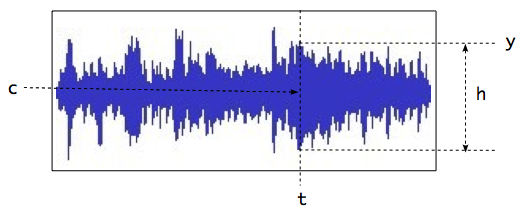
\includegraphics[width=90mm]{imgs/graph}
 \caption{A simple graphic signal, defined at time t by a coordinate y, a thickness h and a color c}
 \label{graphimg}
\end{figure}

%-------------------------------
%:    The signal static node.
\sublevel{The 'signal' static node.}
A \OSC{scene} includes a static signal node, which OSC address is \OSC{/ITL/\textit{scene}/signal} which may be viewed as a container for signals. It is also used for \textit{composing signals in parallel}.

The \OSC{signal} node supports only the \OSC{get} message that gives the list of the defined signals.

\example \\
Querying the signal node:
\sample{/ITL/scene/signal get;}
\sampleindent will give the enclosed signals definitions:
\sample{/ITL/scene/signal/y size 200 ;\\
/ITL/scene/signal/h size 200 ;
}


\subsublevel{Signal messages.}
\label{ssignal}
Signal messages can be sent to any address with the form \OSC{/ITL/\textit{scene}/signal/\textit{identifier}}, where \OSC{\textit{identifier}} is a unique signal identifier.
The set of messages supported by a signal is the following:
\begin{rail}
simpleSignal : [1] ( float32 + )
		| [2] ('size' int32) 
		| [3] ('default' float32)
		| [4] 'get' ( | 'size' | 'default')
		| [5] 'reset'
		| [6] 'del'
\end{rail}
\index{signal}
\index{signal!simple signal!size}
\index{signal!simple signal!default}
\index{signal!simple signal!get}
\index{signal!simple signal!reset}
\index{signal!simple signal!del}

\begin{itemize}
\item \textbf{[1]} push an arbitrary data count into the signal buffer. The expected data range is \values{[-1,1]}. Note that the internal data buffer is a ring buffer, thus data are wrapped when the data count if greater than the buffer size. 
\item \textbf{[2]} the \OSC{size} message sets the signal buffer size. When not specified, the buffer size value is the size of the first data message. 
\item \textbf{[3]} the \OSC{default} message sets the \emph{default signal value}. A signal \emph{default value} is the value returned when a query asks for data past the available values.
\item \textbf{[4]} the \OSC{get} message without parameter gives the signal current values. The \OSC{size} and  \OSC{default} parameters are used to query the signal size and default values.
\item \textbf{[5]} the \OSC{reset} message clears the signal data. 
\item \textbf{[6]} the \OSC{del} message deletes the signal from the \OSC{signal} space. Note that it is safe to delete a signal even when used by a graphic signal. 
\end{itemize}

\example \\
Creating a signal with a given buffer size:
\sample{/ITL/scene/signal/mySig size 200;}
Creating a signal with a given set of data (the buffer size will be the data size):
\sample{/ITL/scene/signal/mySig 0.\ 0.1\ 0.2\ 0.3\ 0.4\ 0.5\ 0.4\ 0.3\ 0.2\ 0.1\ 0.\ -0.1\ -0.2 ;}


%-------------------------------
%:    Composing signals in parallel.
\subsublevel{Composing signals in parallel.}\label{parcomp}
Composing signals in parallel produces a signal which value at a time \values{t} is a vector of the composed signals values. Thus an additional read-only attribute is defined on \emph{parallel signals} : the signal \emph{dimension} which is size of the signals vector. Note that the dimension property holds also for simple signals.

The format of the messages for parallel signals is the following:
\begin{rail}
parallelSignal :  
		  [1] 'set' ( signal + )
		| [2] (| projectionString) ( float32 + )
		| [3] ('get' 'dimension') 
\end{rail}
\index{signal!parallel signal}
\index{signal!parallel signal!get}
where 
\begin{rail}
signal :  
		  [4] identifier
		| [5] float32
\end{rail}

\begin{itemize}
\item \textbf{[1]} defines a new signal composed of the signals given as parameters. A signal parameter is defined as:

\begin{itemize}
\item \textbf{[4]} an \OSC{identifier} i.e. a signal name referring to an existing signal in the \OSC{signal} node. 
\item \textbf{[5]} or as a float value. This form is equivalent to an anonymous constant signal holding the given value. 
\end{itemize}

\item \textbf{[2]} sets the values of the signals using a projection string. See section \fullref{sigproj}. 
\item \textbf{[3]} in addition to the \OSC{get} format defined for signals, a parallel signal supports the \OSC{get dimension} message, that gives the number of simple signals in parallel. The dimension of a simple signal is 1. 
\end{itemize}

\example \\
Putting a signal \OSC{y} and constant signals 0.01 0. 1. 1. 1. in parallel:
\sample{/ITL/scene/signal/mySig set y 0.01 0. 1. 1. 1. ;}
Querying the previously defined parallel signal:
\sample{/ITL/scene/signal/mySig get ;\\
will give the following output: \\
/ITL/scene/signal/mySig set y 0.01 0. 1. 1. 1.
}

\note{} \\
For a parallel signal:
\begin{itemize}
\item the \OSC{get size} message gives the maximum of the components size. 
\item the \OSC{get default} message gives the default value of the first signal. 
\end{itemize}

%-------------------------------
%:    Distributing data to signals in parallel
\subsublevel{Distributing data to signals in parallel}
\label{sigproj}

When signals are in parallel, a \emph{projection string} may be used to distribute data over each signal.
Individual components of a parallel signal may be addressed using a \emph{projection string} that is defined as follows:
\begin{rail}
projectionString :  '[' int32 (| '\~{}' (| int32)) ']'
\end{rail}
\index{signal!parallel signal!projection string}

The projection string is made of a \emph{index value}, followed by an optional \emph{parallel marker} (\OSC{\~{}}), followed by an optional \emph{step value}, all enclosed in brackets.

The \emph{index value} \values{n} is the index of a target signal. When the \emph{parallel marker} option is not present, the values are directed to the target signal. Indexes start at 0.

\example \\
Sending data to the second component of a parallel signal:
\sample{/ITL/scene/signal/sig '[1]' 0.\ 0.1\ 0.2\ 0.3\ 0.4\ 0.5\ 0.4\ 0.3\ 0.2\ 0.1\ 0. ;}
\sampleindent is equivalent to the following message (assuming that the second signal name is 's2'):
\sample{/ITL/scene/signal/s2 0.\ 0.1\ 0.2\ 0.3\ 0.4\ 0.5\ 0.4\ 0.3\ 0.2\ 0.1\ 0. ;}

Note that:
\begin{itemize}
\item the message is ignored when \values{n} is greater than the number of signals in parallel. Default \values{n} value is \values{0}. 
\item setting directly the values of a simple signal or as the projection of a parallel signal are equivalent.
\end{itemize}

The \emph{parallel marker} (\OSC{\~{}}) and the \emph{step value} \values{w} options affect the target signals. Let's consider \values{s[n]} as the signal at index \values{n}. The values are distributed in sequence and in loop to the signals \values{s[n], s[n+w]...s[m]} where \values{m} is the greatest value of the index \values{n+(w.i)} that is less than the signal dimension. The default  \emph{step value} is \values{1}.

\example \\
Sending data to the second and third components of a set of 3 parallel signals:
\sample{/ITL/scene/signal/sig [1\~{}] 0.1 0.2 ;}
\sampleindent is equivalent to the following messages (assuming that the signal dimension is 3):
\sample{/ITL/scene/signal/sig [1] 0.1 ;\\
/ITL/scene/signal/sig [2] 0.2 ;
}
\sampleindent or to the following (assuming that the target signal names are 's2' and 's3'):
\sample{/ITL/scene/signal/s2 0.1;\\
/ITL/scene/signal/s3 0.2;
}


%---------------------------------
%: signal connections
\sublevel{Connecting signals to graphic attributes.}
\label{signalcnx}

A signal may be connected to one or several graphic attributes of an object. Only the common attributes  (see section \fullref{common}) support this mechanism.
When a connection between a signal and an object attribute is set, sending values to the signal is equivalent to send the values to the connected object attribute. A similar behavior could be achieved by sending the equivalent messages, however the connection mechanism is provided for efficiency reasons and in addition, it supports values scaling. 

\begin{rail}
signalcnx : 	( 'connect'   connection )
			| 	'disconnect' ( [1] connection | [2] signal | [3]  signal object )
\end{rail}
\index{signal!connect}
\index{signal!disconnect}

\begin{itemize}
\item the \OSC{connect} message makes a connection between a signal and one or several attributes of one or several objects.
\item the \OSC{disconnect} message breaks a specific connection \textbf{[1]} or all the connections of a given signal \textbf{[2]}, or all connections between a given signal and a given object \textbf{[3]}.
\end{itemize}

\begin{rail}
connection : signal ( target + )
\end{rail}
\index{signal!connection}
\begin{itemize}
\item \OSC{signal} is a name referring to an existing component of the \OSC{signal} node. 
\end{itemize}

\begin{rail}
target :  object ( ':' attribute ( | '[low,high]' ) + )
\end{rail}
\begin{itemize}
\item \OSC{object} is the name of an object (must be on the same hierarchy level than the \OSC{signal} node).
\item \OSC{attribute} is the name of the object target attribute (same name as the method used to set the attribute, e.g. \OSC{x}, \OSC{angle}, etc.).
\item an optional scaling feature is provided with the \OSC{[low,high]} suffix: signal values are expected to be between -1 and 1, the scaling suffix re-scale the input values between \OSC{low} and \OSC{high}.
\end{itemize}

\note{} \\
Connections are restricted to one-dimensional signals as source and to one-dimensional attribute as target. This is not a real limitation since any component of a multi dimensional attribute (e.g. \OSC{color}) is always available as a single attribute (e.g. \OSC{red} or \OSC{blue}).

\note{} \\
A connection can't cross the borders of a component i.e. the target object and the signal node should have the same parent.

\example \\
Connecting signals to attributes:
\sample{! connects the values of sig1 to the red attribute of the 'rect' object \\
/ITL/scene/signal connect sig1 "rect:red"; \\
! connects the values of sig2 to several objects and attributes \\
/ITL/scene/signal connect sig2 "rect:blue:x:rotatey[0,360]" "cursor:date[0,15]";}
Disconnecting some of the previous connections :
\sample{/ITL/scene/signal disconnect sig2 "cursor:date" "rect:rotatey:blue"; }

%-------------------------------
%:    Graphic signals.
\sublevel{Graphic signals.}
\label{gsignal}

A graphic signal is the graphic representation of a set of parallel signals. It is created in the standard scene address space. A simple graphic signal is defined by a parallel signal controling the \values{y} deviation value, the thickness and the color at each time position. The color is encoded as HSBA colors (Hue, Saturation, Brightness, Transparency). The mapping of a signal value  (\values{[-1,1]}) to the HSBA color space is given by the table \ref{hsbamap}. 

\begin{figure}[h]
	\centering 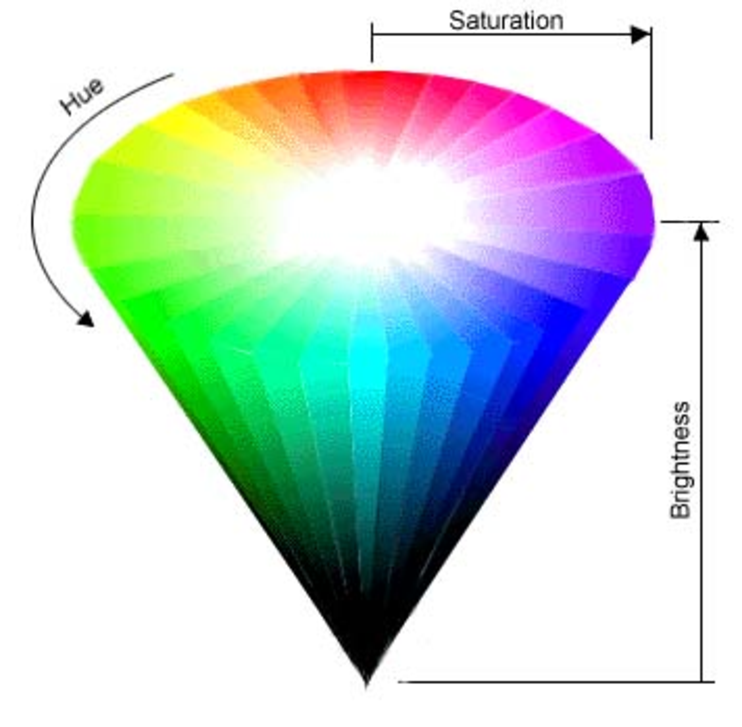
\includegraphics[width=65mm]{imgs/hsb}
 \caption{The HSB color space}
 \label{hsbfiug}
\end{figure}


\begin{table}[htdp]
\caption{HSBA color values.}
\begin{center}
\begin{tabular}{|r|cl|}
\hline
parameter & mapping & \\
\hline
\OSC{hue}				& \OSC{[-1,1]} & corresponds to \OSC{[-180,180]} angular degree where \OSC{0} is red. \\
\OSC{saturation}		& \OSC{[-1,1]} & corresponds \OSC{0\%} to \OSC{100\%} saturation. \\
\OSC{brigthness}		& \OSC{[-1,1]} & corresponds \OSC{0\%} (black) to \OSC{100\%} (white) brithgness. \\
\OSC{transparency}		& \OSC{[-1,1]} & corresponds \OSC{0\%} to \OSC{100\%} tranparency. \\
\hline
\end{tabular}
\end{center}
\label{hsbamap}
\end{table}



A graphic signal responds to common component messages (section \fullref{common}). Its specific messages are the following:
\begin{rail}
graphicSignal : 'set' 'graph' signalIdentifier 
			| 'get' 'dimension'
\end{rail}
\index{Graphic signal!set}
\index{Graphic signal! dimension}

\begin{itemize}
\item the \OSC{set} message is followed by the \OSC{graph} type and a \OSC{\textit{signalIdentifier}}, where \OSC{signalIdentifier} must correspond to an existing signal from the \OSC{signal} address space. In case \OSC{signalIdentifier} doesn't exist, then a new signal is created at the \OSC{signalIdentifier} address with default values. 
\item the \OSC{get dimension} message gives the number of graphic signals in parallel (see section \fullref{pgsignal}). 
 \end{itemize}
 
\example \\
Creating a signal and its graphic representation:
\sample{/ITL/scene/signal/y size 200 ; \\
! use of constant anonymous signals for thickness and color\\
/ITL/scene/signal/sig set y 0.1 0. 1. 1. 1. ; \\
/ITL/scene/siggraph set graph sig ;
}

%-------------------------------
%:    Graphic signal default values.
\subsublevel{Graphic signal default values.}
As mentionned above, a graphic signal expects to be connected to parallel signals having at least an \values{y} component, a graphic thickness component and HSBA components. Thus, from graphic signal viewpoint, the expected dimension of a signal should be equal or greater than 6. In case the \OSC{signalIdentifier} dimension is less than 6, the graphic signal will use the default values defined in table \ref{gsigdefault}.

\begin{table}[htdp]
\caption{Graphic signal default values.}
\begin{center}
\begin{tabular}{|r|cl|}
\hline
parameter & default value & \\
\hline
\OSC{y}					& \OSC{0} & the center line of the graphic \\
\OSC{thickness}		& \OSC{0} & \\
\OSC{hue}				& \OSC{0} & meaningless due to brigthness value \\
\OSC{saturation}		& \OSC{0} & meaningless due to brigthness value \\
\OSC{brigthness}		& \OSC{-1} & black \\
\OSC{transparency}		& \OSC{1} & opaque \\
\hline
\end{tabular}
\end{center}
\label{gsigdefault}
\end{table}

%-------------------------------
%:    Parallel graphic signals.
\subsublevel{Parallel graphic signals.}
\label{pgsignal}
When the dimension \textit{d} of a signal connected to a graphic signal is greater than 6, then the input signal is interpreted like parallel graphic signals. More generally, the dimension \textit{n} of a graphic signal is:
\[
n  \  |\ n \in \mathbb{N}\ \land\ 6.(n-1) < d \leqslant 6.n
\]
where \textit{d} is the dimension of the input signal.

When \textit{d} is not a mutiple of 6, then the last graphic signal makes use of the default values mentionned above.

 
\example \\
Creating parallel graphic signals:
\sample{/ITL/scene/signal/y1 size 200 ; \\
/ITL/scene/signal/y2 size 200 ; \\
! use of constant anonymous signals for thickness and color\\
/ITL/scene/signal/sig1 set y1 0.1 0. 1. 1. 1. ; \\
! use a different color for 'sig2'\\
/ITL/scene/signal/sig2 set y2 0.1 0.6 1. 1. 1. ; \\
! put 'sig1' and 'sig2' in parallel\\
/ITL/scene/signal/sig set sig1 sig2;    \hspace{1CM}! 'sig' dimension is 12\\
/ITL/scene/siggraph set graph sig; 
}

\note{} \\
Using data projection may be convenient when the input signal represents interleaved data. For example, the projection string \OSC{[n\~{}6]} distribute data over similar components of a set of graphic signals, where \OSC{n} represents the index of the graphic signal target component.


%===============================
%:Events and Interaction
\toplevel{Events and Interaction}
\label{interaction}

Interaction messages are user defined messages associated to events and triggered when these events occur. These messages accept variables as message arguments.

The general form of the message is the following:
\begin{rail}
interactMsg : (('watch' | 'watch+')  ([1] | 
					what  ( [2] 
							| [3] "(" ( ( message  )+ "," ) ")" 
							| [4] message )  )) 
\end{rail}
\index{Interaction!watch}
\index{Interaction!watch+}

\OSC{what} represents the event to watch and \OSC{message} is a list of associated messages, separated by a comma. 

\begin{itemize}
\item [1]: clear all the messages for all the events.
\item [2]: clear the messages associated to the \OSC{what} event.
\item [3]: associate a list of messages to the \OSC{what} event. With \OSC{watch}, the messages replace previously associated messages. Using \OSC{watch+}, the messages are appended to the messages currently associated to the event.
\item [4]: associate or add a single message to the \OSC{what} event. This form is provided for compatibility with previous versions.
\end{itemize}

\note{} \\
	The [1] and [2] form has no effect with the \OSC{watch+} message. \\
	In some environments, the comma has a special meaning, making tricky to use it as a message separator. This is why ':' is also accepted as separator in OSC messages.

\begin{rail} 
message : (| addressPrefix)  OSCAddress ( | (parameters | variable) + )
\end{rail}

The associated messages are any valid OSC message (not restricted to the INScore message set), with an extended address scheme, supporting IP addresses or host names and udp port number to be specified as OSC addresses prefix. The message parameters are any valid OSC type or variable (see section \ref{interactvar}).


\begin{rail} 
addressPrefix : (IPAddress | hostname) ':' port
\end{rail}

\example \\
An extended address to send messages to \OSC{localhost} on port \OSC{12000}:
\sample{localhost:12000/your/osc/address;}

%===============================
%:    Events
\sublevel{Events}
\label{defevents}


%===============================
%:       UI events
\subsublevel{UI events}
\label{uievents}

User interface events are typical mouse events:
\begin{rail}
what : 'mouseDown' | 'mouseUp' | 'mouseEnter' | 'mouseLeave' | 'mouseMove' | 'doubleClick' 
\end{rail}
\index{Interaction!Events!mouseDown}
\index{Interaction!Events!mouseUp}
\index{Interaction!Events!mouseEnter}
\index{Interaction!Events!mouseLeave}
\index{Interaction!Events!mouseMove}
\index{Interaction!Events!doubleClick}
	
\example \\
Triggering a message on mouse down:
\sample{/ITL/scene/myObject watch mouseDown (/ITL/scene/myObject show 0);}
\sampleindent the object hides itself on mouse click. \\
Triggering a message on mouse down but addressed to another host on udp port 12100:
\sample{/ITL/scene/myObject watch mouseDown (host.domain.org:12100/an/address start); }

\note{} \\
UI events are not supported by objects that are synchronized as slave.

Mouse events can be simulated using a \OSC{event} message:
\begin{rail}
uievt : 'event' mouseEvent x y
\end{rail}
\index{Interaction!Events!event}
where \OSC{mouseEvent} is one of the events described above, \OSC{x} and \OSC{y} are integer values giving the click position, expressed in pixels and relative to the target object.

\example \\
Simulating a mouse down at position 10, 10 :
\sample{/ITL/scene/myObject event mouseDown 10 10;}


%===============================
%:       Time events
\subsublevel{Time events}
\label{timeevents}

Events are also defined on the time domain:
\begin{rail}
what : 	'timeEnter' time time | 'timeLeave' time time 
		| 'durEnter' time time | 'durLeave' time time 
\end{rail}
\index{Interaction!Events!timeEnter}
\index{Interaction!Events!timeLeave}
\index{Interaction!Events!durEnter}
\index{Interaction!Events!durLeave}

Each event takes a time interval as parameter, defined by two \OSC{time} specifications (see section \fullref{time} for the time format)

\begin{itemize}
\item \OSC{timeEnter}, \OSC{timeLeave} are triggered when an object date is moved to or out of a watched time interval,
\item \OSC{durEnter}, \OSC{durLeave} are triggered when an object duration is moved to or out of a watched time interval.
\end{itemize}

\example \\
An object that moves a score to a given page number when it enters its time zone.
\samplev{/ITL/scene/myObject watch timeEnter 10/1 18/1 (/ITL/scene/score page 2);}


%===============================
%:       Miscellaneous events
\subsublevel{Miscellaneous events}
\label{miscevents}

\begin{rail}
what : 	  'export'
		| 'newElement'
		| 'endPaint'
		| 'del'
\end{rail}
\index{Interaction!Events!export}
\index{Interaction!Events!newElement}
\index{Interaction!Events!endPaint}
\index{Interaction!Events!del}

\begin{itemize}
\item the \OSC{export} event is supported by all the components. It is triggered after an export message has been handled and could be used to simulate synchronous exports.
\item the \OSC{newElement} event is supported at scene level only and triggered when a new element is added to the scene.
\item the \OSC{endPaint} event is supported at scene level only and triggered after a scene has been painted.
\item the \OSC{del} event is triggered when an object is being deleted.
\end{itemize}

\example \\
Displaying a welcome message to new elements:
\sample{/ITL/scene watch newElement (/ITL/scene/msg set txt "Welcome");}

%===============================
%:    Variables
\sublevel{Variables}
\label{interactvar}

Variables are values computed when an event is triggered. These values are send in place of the variable. A variable name starts with a '\$' sign. 

%===============================
\subsublevel{Position variables}
\label{posvar}

Position variables reflects the current mouse position for mouse events. They are set to \values{0} for the other events. 

\begin{rail} 
posVar : xy | 'absx' | 'absy' | 'sx' | 'sy' 
\end{rail}
\index{Interaction!variable!x}
\index{Interaction!variable!y}
\index{Interaction!variable!absx}
\index{Interaction!variable!absy}
\index{Interaction!variable!sx}
\index{Interaction!variable!sy}

where
\begin{rail} 
xy : ('x' | 'y') ( | '[low,high]') 
\end{rail}

\begin{itemize}
\item \OSC{\$x} \OSC{\$y}: denotes the mouse pointer position at the time of the event. The values are in the range \values{[0,1]} where 1 is the object size in the x or y dimension. The value is computed according to the object origin: it represents the mouse pointer distance from the object x or y origin (see \fullref{origin}). \OSC{\$x} and \OSC{\$y} variables support an optional range in the form \OSC{[low, high]} that transforms the \values{[0,1]}  values range into the \values{[low, high]} range.

\item \OSC{\$absx} \OSC{\$absy}: denotes the mouse pointer absolute position at the time of the event. The values represent a pixel position relative to the top-left point of the target object. Note that this position is unaffected by scale. 
Note also that the values are not clipped to the object dimensions and could exceed its width or height or become negative in case of mouse move events.

\item \OSC{\$sx} \OSC{\$sy}: denotes the mouse pointer position in the scene coordinates space. 
\end{itemize}

\example \\
An object that follows mouse move.\\
\sample{/ITL/scene/myObject watch mouseDown ( \\
\hspace*{3cm}/ITL/scene/myObject x '\$sx', \\
\hspace*{3cm}/ITL/scene/myObject y '\$sy' );}


%===============================
\subsublevel{Time variables}
\label{timevar}

Time variables reflects the date corresponding to the current mouse position for mouse events. 
They are set to \values{0} for the other events. 

\begin{rail} 
timeVar :  ('date' | 'rdate') (| ':'  mapname) (| '[n/d]') (| '\%' 'f')
\end{rail}
\index{Interaction!variable!date}
\index{Interaction!variable!rdate}

\begin{itemize}
\item \OSC{\$date}: denotes the object date corresponding to the mouse pointer position at the time of the event. It is optionnaly followed by a colon and the name of the mapping to be used to compute the date. The \OSC{\$date} variable is replaced by its rational value (i.e. two integers values). The optional rational enclosed in brackets may be used to indicate a quantification: the date value is rounded to an integer count of the specified rational value. The optional \OSC{\%f} may be used to get the date delivered as a float value.
\item \OSC{\$rdate}: is similar to \OSC{\$date} but ignores the target current date: the date is relative to the object mapping only.
\end{itemize}

\note{} \\
A variable can be used several times in a message, but several \OSC{\$date} variables must always refer to the same mapping.

\example \\
Sending the current date as a float value to an external application:\\
\sample{/ITL/scene/myObject watch mouseDown ( targetHost:12000/date '\$date\%f' );}

%===============================
\subsublevel{Miscellaneous variables}
\label{miscvar}

\begin{rail} 
variable :  'name' | 'scene' | 'address'
\end{rail}
\index{Interaction!variable!scene}
\index{Interaction!variable!name}
\index{Interaction!variable!address}

\begin{itemize}
\item \OSC{\$name} is replaced by the target object name.
\item \OSC{\$scene} is replaced by the target object scene name.
\item \OSC{\$address} is replaced by the target object OSC address. 
\end{itemize}

\note{} \\
For the \OSC{newElement} event, the target object is the new element. 

\example \\
Using an object name:
\sample{/ITL/scene watch newElement (/ITL/scene/welcome set txt "Welcome" '\$name');}

%===============================
%:    Message based variables
\subsublevel{Message based variables}
\label{msgvar}

A message based variable is a variable containing an OSC message which will be evaluated at the time of the event. They are supported by all kind of events. Like  the variables above, a message based variable starts with a '\$' sign followed by a valid 'get' message enclosed in parenthesis:
\begin{rail} 
msgVar : '(' oscaddress 'get' (| params) ')'
\end{rail}

The evaluation of a 'get' message produces a message or a list of messages. The message based variable will be replaced by the parameters of the messages resulting from the evaluation of the 'get' message.
Note that all the 'get' messages attached to an event are evaluated at the same time.

\example \\
An object that takes the \values{x} position of another object on mouse down:
\sample{/ITL/scene/myObject watch mouseDown \\
\hspace*{3cm}(/ITL/scene/myObject x '\$(/ITL/scene/obj get x)');}


%===============================
%:    OSC address variables
\subsublevel{OSC address variables}
\label{oscvar}
The OSC address of a message associated to an event supports the following variables:
\begin{itemize}
\item \OSC{\$self}: replaced by the object name.
\item \OSC{\$scene}: replaced by the scene name.
\end{itemize}

\example \\
Requesting a set of objects to send a message to themselves on a mouse event:
\sample{/ITL/scene/* watch mouseDown \hspace*{2.4cm}! request all the objects of the scene \\
\hspace*{2.7cm}(/ITL/scene/\$self x '\$sx'); ! to send a message to themselves
}

%===============================
%:    Interaction state management
\sublevel{Interaction state management}
\label{evtstate}

For a given object, its \emph{interaction state} (i.e. the watched events and the associated messages) can be saved and restored.
\begin{rail} 
stateMsg : 'push' | 'pop'
\end{rail}
\index{Interaction!push}
\index{Interaction!pop}

Interaction states are managed using a stack where the states are pushed to or popped from.
\begin{itemize}
\item \OSC{push}: push the current interaction state on top of the stack.
\item \OSC{pop}: replace the current interaction state with the one popped from the top of the stack.
\end{itemize}

The different states stored in this stack can be obtain with the message :

\begin{rail} 
stackMsg : 'get' 'stack'
\end{rail}

\note{} \\
The effect of a pop message addressed to an object with an empty stack is to clear the object current interaction state.


%===============================
%:    File watcher
\sublevel{File watcher}
\label{filewatch}

The \OSC{fileWatcher} is a static node of a scene that is intended to watch file modifications. \\
It receives messages at the address \OSC{/ITL/scene/fileWatcher}.

The \OSC{fileWatcher} support the \OSC{watch} and \OSC{watch+} messages as described in section \fullref{interaction} with a file name used in place of the \OSC{what} parameter.

\begin{rail}
fileWatcher : (('watch' | 'watch+')  ( | filePath  ( |  ( ( message  )+ "," ) )  )) 
\end{rail}
\index{fileWatcher!watch}
\index{fileWatcher!watch+}

\example \\
Reload aa INScore script on file modification:
\sample{
/ITL/scene/fileWatcher wach 'myScript.inscore' \\
\hspace*{3cm}( /ITL/scene load 'myScript.inscore' );
}

%\sublevel{Debug}
%
%Each object has a \OSC{debug} sub-node for debugging purposes. This \OSC{debug} virtual node has 3 flags, that can be actived or desactived with \OSC{0} or \OSC{1}:
%
%\begin{rail}
%debug : 		('name'  int32)
%		|	('map' int32)
%		|	('signal' int32)
%\end{rail}
%
%\begin{itemize}
%\item When the \OSC{name} flag is on, each scene component displays its bounding rectangle and name.
%\item When the \OSC{map} flag is on, each scene component displays its mappings.
%\item When the \OSC{signal} flag is on, each object (even the scene or the application) will, according to its type, emit 'performance related' signals (or no signal). This 'performance signal' is specific to the type of object. The name of 'performance signal' is of the form \OSC{debug-}\emph{objectName}\OSC{-}\emph{SomeName}. Currently, only the \OSC{application}, the \OSC{scene} and \OSC{graph} objects emit 'performance signals'.
%\end{itemize}



%===============================
%:Scripting
\toplevel{Scripting}
\label{scripting}

INScore saves its state to files containing textual OSC messages. These files can be edited or created from scratch using any text editor. In order to provide users with a scripting language, the OSC syntax has been extended at textual level.

%===============================
%:    Statements
\sublevel{Statements}\label{scriptstatement}
An INScore file is a list of textual expressions. A script expression is:
\begin{itemize}
\item a message: basically a textual OSC message extended to support URL like addresses and variables as parameters.
\item a variable declaration.
\item a foreign language script that may generate messages as output.
\end{itemize}

\begin{rail}
expression :  
		 	message ";"
		| 	variabledecl ";"
		| 	script
\end{rail}
\index{Scripting!expressions}

Messages and variables declarations must be followed by a semicolon, used as statements separator.

%===============================
%:    Messages
\sublevel{Messages}\label{scriptmsgs}

Messages are basically OSC messages that support the address extension scheme described in section \fullref{interaction}.
Thus a script may be designed to initialize an INScore scene and external applications as well, including on remote hosts.

\example\\
Initializing a score and an external application listening on port 12000 and running on a remote host named \OSC{host.adomain.net}.
\sample{/ITL/scene/score set gmnf 'myscore.gmn';\\
host.adomain.net:12000/run 1;
}

Messages parameters can be replaced by variables that are evaluated at parsing level. Variables are described in section \ref{scriptvar}.

%===============================
%:    types
\sublevel{Types}\label{scripttypes}

Using OSC, the message parameters are typed by the OSC protocol. 
With their textual version, any parameter is converted to an OSC type (i.e. int32, float or string) at parsing level.
A special attention must be given to strings in order to discriminate addresses and parameters. Strings intended as parameters must:
\begin{itemize}
\item be quoted, using single or double quotes. Note that an ambiguous quote included in a string can be escaped using a '\verb+\+'.
\item or make use of the following characters set: \OSC{[-a-zA-Z0-9]+} or \OSC{[\_a-zA-Z][\_a-zA-Z0-9]*}.
 \end{itemize}

\example \\
Different string parameter
\sample{/ITL/scene/text set txt "Hello world";  ! string including a space must be quoted \\
/ITL/scene/img set file 'anImage.png';  ! dots must be quoted too \\
/ITL/scene/foo set txt no\_quotes\_needed;
}


%===============================
%:    Variables
\sublevel{Variables}\label{scriptvar}

A variable declaration associates a name with a list of parameters or a list of messages.
Parameters must follow the rules given in section \ref{scripttypes}. They may include previously declared variables. A message list must be enclosed in parenthesis and a comma must be used as messages separator.
\begin{rail} 
variabledecl : 'ident' '=' ( (param | variable) +
					| '(' (message + ',') ')' ) ';'
\end{rail}
\index{Scripting! variable}

\example \\
Variables declarations
\sample{color = 200 200 200; \\
colorwithalpha = \$color 100; ! using another variable \\
msgsvar= ( \hspace*{2.7cm}  ! a variable refering to a message list \\
\hspace*{1cm} localhost:7001/world "Hello world", \\
\hspace*{1cm} localhost:7001/world "how are you ?" );
}


A variable may be used in place of any message parameter. A reference to a variable must have the form \OSC{\$ident} where \OSC{ident} is a previously declared variable. A variable is evaluated at parsing level and replaced by its content.

\example \\
Using a variable to share a common position:
\sample{x = 0.5;\\
/ITL/scene/a x \$x;\\
/ITL/scene/b x \$x;
}

Variables can be used in interaction messages as well, which may also use the variables available in the interaction context (see section \fullref{interactvar}). To differentiate between a \emph{script} and an \emph{interaction} variable, the latter must be quoted to be passed as strings and to prevent their evaluation by the parser. 

\example \\
Using variables in interaction messages: \$sx is evaluated at event occurrence	and \$y is evaluated at parsing level.
\sample{y = 0.5;\\
/ITL/scene/foo watch mouseDown (/ITL/scene/foo "\$sx" \$y);
}


%===============================
%:    Message based parameters
\sublevel{Message based parameters}\label{scriptmsgparam}

Similarly to message based variables (see section \fullref{msgvar}), a message parameter may also use the result of a \OSC{get} message as parameters specified like a message based variable.
The message must be enclosed in parameters with a leading \$ sign.
\begin{rail} 
msgparam : '(' (message) ')'
\end{rail}
\index{Scripting! message based parameters}

\example \\
Displaying INScore version using a message parameter:
\sample{/ITL/scene/version set  txt "INScore version is" \$(/ITL get version);}

\note{}\\
Message based parameters are evaluated by the parser. Thus when the system state is modified by a script before a message parameter, these modifications won't be visible at the time of the parameter evaluation because all the messages will be processed by the next time task. For example:\\
\sample{/ITL/scene/obj x 0.1;\\
/ITL/scene/foo x \$(/ITL/scene/foo get x);}
x position of \OSC{/ITL/scene/foo} will be set to x position of \OSC{/ITL/scene/obj} at the time of the script evaluation (that may be different to 0.1).

%===============================
%:    languages
\sublevel{Languages}\label{scriptlang}

\index{Scripting!javascript}
\index{Scripting!lua}

INScore supports Javascript and Lua as scripting languages. Javascript is embedded by default (using the v8 engine\footnote{\url{http://code.google.com/p/v8/}}). INScore needs to be recompiled to embed the Lua engine\footnote{\url{http://www.lua.org/}}. A script section is indicated similarly to a Javascript section in html i.e. enclosed in an opening \OSC{<?} and a closing \OSC{?>}.
\begin{rail} 
script : '<?' ('javascript' | 'lua') script '?>'
\end{rail}
\index{Scripting! javascript}
\index{Scripting! lua}

The principle of using an embedded programming language in script files is the following: \emph{javascript} or \emph{lua} sections are given to the corresponding engine and are expected to produce INScore messages on output.
These messages are then parsed as if replacing the corresponding script section.

Note that INScore variables are exported to the current language environment.

\example
\sample{
<?javascript \\
\hspace*{3mm} "/ITL/scene/version set 'txt' 'Javascript v."  + version() + "';"; \\
\hspace*{1mm} ?>
}


A single persistent context is created at application level and for each scene.
It allows scripts to reuse previously defined functions and thus to design more structured scripts.


%===============================
%:    The Javascript objects
\subsublevel{The Javascript object}\label{jsobj}

The Javascript engine is available at runtime at the address \OSC{/ITL/\textit{scene}/javascript}. It has a \OSC{run} method that takes a javascript string as parameter.

\begin{rail} 
javascript :  'run' 'code'
\end{rail}
\index{Scripting! javascript! run}

The \OSC{run} method evaluates the code. Similarly to javascript sections in scripts, the output of the evaluation is expected to be a string containing valid INScore messages that are next executed. 
Actually, including a javascript section in a script is equivalent to send the \OSC{run} message with the same code as parameter to the javascript object.

The Javascript engine is based on V8 that implements ECMAScript as specified in ECMA-262, 5th edition, extended with additional functions:
\begin{itemize}
\item \textbf{\OSC{version()}} : gives the javascript engine version number as a string.
\item \textbf{\OSC{print(val1 [, val2 [, ...]])}} : print the arguments to the OSC standard output. The arguments list is prefixed by 'javascript:'. The function is provided for debug purpose.
\item \textbf{\OSC{readfile(file)}} : read a file and returns its content as a string. The file name could be specified as an absolute or relative path. When relative, the file is searched in the application current \OSC{rootPath} (see section \fullref{applmgmt}).
\item \textbf{\OSC{post(address [,...])}} : build an OSC message and post it for delayed processing i.e. to be processed by the next time task. \OSC{address} is an OSC or an extended OSC address. Optional arguments are the message parameters.
\end{itemize}


\example
\sample{
<?javascript \\
\hspace*{3mm} post ("/ITL/scene/obj", "dalpha", -1);";\\ 
\hspace*{3mm} The message /ITL/scene/obj dalpha -1 \\
\hspace*{3mm} will be evaluated by the next time task. \\
?>
}


%\note{}\\
%The effect of \OSC{load} message is actually to push the messages on the system stack for evaluation by the next time task. Thus when including a file containing javascript (or lua), the new 
%language context won't be available to the next messages in the script. The workaround 
%for structured script consists in designing a top level script that only contains \OSC{load} messages.
%
%\example
%\sample{
%\hspace*{-3mm} /ITL load 'javascript-code.inscore';\\
%/ITL load 'call-javascript.inscore';
%}


%===============================
%:Plugins
\toplevel{Plugins}
\label{plugins}

A plugin is an external library that is dynamically loaded when an object that need it is created.
The system looks for plugins in the following locations:
\begin{itemize}
\item in the current folder first
\item in the PlugIns folder, located in the application bundle on macos, in the application folder on other systems
\item in the system default locations for shared libraries
\end{itemize}
Additionaly, a user path can be set, where the system will look for plugins in first position. See section \fullref{ITLplugins}.

The plugins are shared libraries which extension is platform dependent. The plugin name should not include the extension. The expected extensions are the following: .dylib on MacOS and Linux, .dll on Windows.



%===============================
%:   FAUST plugins
\sublevel{FAUST plugins}
\label{faust}

FAUST [Functional Audio Stream]\footnote{\url{http://faust.grame.fr}} is a functional programming language specifically designed for real-time signal processing and synthesis. A FAUST/INScore architecture allows to embed FAUST processors in INScore, for the purpose of signals computation. A FAUST plugin is viewed as a parallel signal and thus it is created in the \OSC{signal} address space. Similarly to signals, it is associated to an OSC address in the form \OSC{/ITL/\emph{scene}/signal/\emph{name}} where \OSC{\emph{name}} is a user defined name.

\subsublevel{Set Message}

There are two ways to create a FAUST Processor : 
\begin{itemize}
\item [1]- By charging a DSP as a plugin already compiled \\

\begin{rail}
faustprocessor : 'set' 'faust' path
\end{rail}
\index{faustprocessor!set}

\example \\
\sample{/ITL/scene/signal/myFaust set faust aFaustPlugin;}

\note{} \\
The plugin name should not include the extension. The expected extensions are the following: .dylib on MacOS and Linux, .dll on Windows. \\

\item [2]- By charging libfaust as a plugin to compile a DSP on-the-fly  (as a string or a file). \\
\begin{rail}
faustdsp : 'set' 'faustdsp' faustcode
\end{rail}
\index{faustprocessor!set}

\vspace{0.3cm}

\begin{rail}
faustdspfile : 'set' 'faustdspf' faustfile
\end{rail}
\index{faustprocessor!set}

\example \\
\sample{/ITL/scene/signal/plus set faustdsp "process=+;"; \\
/ITL/scene/signal/mydsp set faustdspf "mydsp.dsp";
}

\end{itemize}

%===============================
%:      Specific messages
\subsublevel{Specific messages}
\label{faustmsg}
A FAUST processor is characterized by the numbers of input and output channels and by a set of parameters. Each parameter carries a name defined by the FAUST processor. The set of messages supported by a FAUST processor is the set of signals messages extended with the parameters names and with specific query messages. 

\begin{rail}
faustmessage : signalMsgs
			 | [1] 'msg' float32
			 | [2] 'get' ('in' | 'out')
\end{rail}
\index{faustprocessor!in}
\index{faustprocessor!out}
\index{faustprocessor!min}
\index{faustprocessor!max}

\begin{itemize}
\item [1] \OSC{\emph{msg}} is any of the FAUST processor parameters, which are defined by the FAUST processor.
\item [2] the \OSC{get} message is extended to query the FAUST processor: \OSC{in} and \OSC{out} give the number of input and output channels.
% \OSC{msgs} gives the list of the processor specific messages under the form of separate messages including the message name followed by its default, minimum and maximum values.
\end{itemize}

\example \\
Querying a FAUST processor input and output count:
\sample{/ITL/scene/signal/myFaust get in out;}
\sampleindent gives as output:
\sample{/ITL/scene/signal/myFaust in 2; \\
/ITL/scene/signal/myFaust out 4;
}
Modifying the value of a FAUST processor parameter named \OSC{volume}:
\sample{/ITL/scene/signal/myFaust volume 0.8}

%===============================
%:      Feeding and composing FAUST processors
\subsublevel{Feeding and composing FAUST processors}
\label{composefaust}

A FAUST processor accepts float values as input, which are taken as interleaved data and distributed to the input channels.

From composition viewpoint, a FAUST processor is a parallel signal which dimension is the number of output channels. 
Thus, a FAUST processor can be used like any parallel signal. However, the signal identifier defined in \ref{parcomp} is extended to support adressing single components of parallel signal as follows:
\begin{rail}
signal :  
		  identifier ( | "/" n)
		| float32
\end{rail}
where \values{n} selects the signal \#n of a parallel signal. Note that indexes start at 0.

\example \\
Creating 3 parallel signals using the 3 output channels of a FAUST processor named \OSC{myFaust}:
\sample{/ITL/scene/signal/y1 set 'myFaust/0' 0.01 0. 1. 1. 1. ;\\
/ITL/scene/signal/y2 set 'myFaust/1' 0.01 0.5 1. 1. 1. ;\\
/ITL/scene/signal/y3 set 'myFaust/2' 0.01 -0.5 1. 1. 1. ;
}


%===============================
%:    Gesture Follower
\sublevel{Gesture Follower}
\label{GF}

INScore supports gesture following using the technology developed by the IRCAM IMTR team. These features are available as a plugin that is included in the INScore distribution (version 1.03 or greater) or available from the IRCAM.
%available from the IRCAM. The plugin installation is documented in the accompanying readme file.

%===============================
%:        Basic principle
\subsublevel{Basic principle}\label{gfbasic}
Gesture following is provided as a mean to interact with a score. From input viewpoint, the gesture follower is similar to signals (see section \fullref{ssignal}): it accepts data stream as input both in learning and following modes. It implements a specific set of events related to gesture following and can generate message streams parametrized with the gesture follower current state.

A gesture follower is setup to handle a given count of gestures, which are actually denoted by streams of float vectors. We'll refer to the size of the float vector as the \emph{gesture dimension}. For example, the dimension of a gesture captured from x, y and z accelerometers is 3.

A gesture follower operates in two distinct phases: a \emph{learning phase} where it actually stores the gestures data, and a \emph{following phase} where it tries to match incoming data to the stored gestures data. When not learning nor following, we'll talk of an idle phase. 

In the \emph{following phase}, the system maintains a list of likelihood for the learned gestures, a list of positions in the gestures and a list of speeds representing how fast the gestures are made. Of course, the higher the likelihood, the more these data are meaningfull. It's the user responsability to decide on the meaningfull likelihood threshold value. Interaction events are triggered only in the \emph{following phase} and for meaningfull likelihoods.

%===============================
%:        Messages
\subsublevel{Messages}\label{gfmessages}
A gesture follower is created in a scene using the \OSC{imtrgf} type. It has a graphic appearance that may be used for debug purpose but it is hidden by default.

\begin{rail}
gesturefollower : 'set' 'imtrgf' gesturedimension bufsize ( name + )
\end{rail}
\index{gesture follower}

The parameters are:
\begin{itemize}
\item \OSC{gesturedimension}: the size of the gestures data vector.
\item \OSC{bufsize}: the size of the gesture data storage.
\item \OSC{name}: a list of names to be used to refer to the learned gestures.
\end{itemize}

\note{} \\
A gesture follower is created with a fixed count of gestures that can be learned and decoded. These gestures are named gestures and can be addressed at \OSC{/ITL/\textit{scene}/\textit{myfollower}/\textit{gesturename}} where the part in italic are user defined names and where \OSC{myfollower} is a gesture follower.


\begin{rail}
gesturefollower :
		  [1] ( float32 + )
		| [2] ('learn' name)
		| [3] 'follow'
		| [4] 'stop'
		| [5] 'clear'
		| [6] ('likelihoodwindow' float32)
		| [7] ('tolerance' float32)
\end{rail}
\index{gesture follower!learn}
\index{gesture follower!follow}
\index{gesture follower!stop}
\index{gesture follower!likelihoodwindow}
\index{gesture follower!tolerance}

\begin{itemize}
\item \textbf{[1]} input data into the gesture follower. The data are interpreted according to the current operating mode i.e. learning, following or idle.
\item \textbf{[2]} starts to learn the gesture designated by \emph{name}. Actually records the next input data to the gesture. 
\item \textbf{[3]} starts following i.e. trying to match the next input data to the recorded gestures.
\item \textbf{[4]} stops learning or following. Actually puts the system in idle phase.
\item \textbf{[5]} clear all the gestures data. This is equivalent to send the \OSC{clear} message to all the gestures. 
\item \textbf{[6]} sets the size of the window that contains the history of the likelihoods. May be viewed as how fast the likelihoods	will change.
\item \textbf{[7]} sets the follower tolerance. 
\end{itemize}

\example \\
Creating a gesture follower for 3 dimensional data and a typical learning sequence:
\sample{/ITL/scene/gf set imtrgf 3 1000 gestureA gestureB gestureC gestureD ;\\
/ITL/scene/gf learn gestureA ;\\
/ITL/scene/gf 0.1 0.5 -0.2 ... 0.7; ! the data size must be a multiple of 3\\
/ITL/scene/gf stop;
}

%===============================
%:        Gestures management
\subsublevel{Gestures management}\label{gfgestures}

Messages can also be sent to gestures i.e. to addresses in the form \OSC{/ITL/\textit{scene}/\textit{myfollower}/\textit{gesturename}} where \OSC{myfollower} is a gesture follower.

A gesture could be in two states:
\begin{itemize}
\item an active state: when its likelihood is greater or equal to the likelihood threshold.
\item an idle state: when its likelihood is lower than the likelihood threshold.
\end{itemize}

\begin{rail}
gesture : 'set' ( float32 +)
		| 'clear'
		| 'learn'
 		| 'likelihoodThreshold' float32
\end{rail}
\index{gesture!set}
\index{gesture!likelihoodThreshold}
\index{gesture!learn}
\index{gesture!clear}


\begin{itemize}
\item \OSC{set}: sets the gesture data. This is equivalent to learn the corresponding data. The \OSC{set} message could be used to restored previously saved gesture data.
\item \OSC{clear}: clears the gesture data. 
\item \OSC{learn}: puts the gestures follower in learning mode and starts learning the corresponding gesture. This is equivalent to send OSC{learn \textit{gesturename}} to the parent gesture follower.
\item \OSC{likelihoodThreshold}: sets the gesture likelihood threshold. The parameter is a float value in the range \values{[0,1]}. Default value is \values{0.5}.
\end{itemize}

Gestures supports also specific queries :
\begin{rail}
gestureget : 'get' (| 'likelihoodThreshold' | 'size')
\end{rail}
\index{gesture!get}
\index{gesture!get!size}

\begin{itemize}
\item \OSC{get}: without parameter, returns a set message when the gesture is not empty.
\item \OSC{size}: gives the current size of the gesture, actually the number of recorded frames. 
\end{itemize}


%===============================
%:        Events and interaction
\subsublevel{Events and interaction}\label{gfevents}

Events are defined at gesture level and events management messages should be addressed to gestures. 

\begin{rail}
gestureevents :
		  	'watch' ( | 'gfEnter' | 'gfLeave' | 'gfActive' | 'gfIdle' )  (  |  messages )
\end{rail}
\index{gesture events!watch}
\index{gesture events!gfEnter}
\index{gesture events!gfLeave}
\index{gesture events!gfActive}
\index{gesture events!gfIdle}

\begin{itemize}
\item \OSC{gfEnter} triggered when the gesture state changes from idle to active.
\item \OSC{gfLeave} triggered when the gesture state changes from active to idle.
\item \OSC{gfActive} triggered in active state each time the gesture likelihood is refreshed.
\item \OSC{gfIdle} triggered in idle state each time the gesture likelihood is refreshed.
\end{itemize}

A message associated to a gesture supports the following specific variables:
\begin{rail}
gesturevariable : 
		( 'gflikelihood'
		| 'gfpos'
		| 'gfspeed') ( | '[low,high]' ) 
\end{rail}
\index{gesture variables!gflikelihood}
\index{gesture variables!gfpos}
\index{gesture variables!gfspeed}
These variables support the scaling feature associated to position variables and described in section \fullref{posvar}.
\begin{itemize}
\item \OSC{gflikelihood} indicates the current likelihood 
\item \OSC{gfpos} indicates the current position in the gesture 
\item \OSC{gfspeed} indicates the current gesture execution speed 
\end{itemize}

\note{}\\
Variables described in section \fullref{interactvar} may also be used but they are meaningless and contains default values.


%===============================
%:        Gesture Follower Appearance
\subsublevel{Gesture Follower Appearance}\label{gfgraphs}

A gesture follower object has a graphic appearance and supports all the standard objects properties, including mapping and synchronization. This graphic appearance is provided mainly for debug purpose and by default, the object is hidden. Figure  \ref{fig:gfgraph} shows the gesture follower appearance in its different phases:
\begin{itemize}
\item when idle, the upper part of the graphic indicates the buffer state of the different gestures. It also includes the gestures likelihood threshold.
\item when learning, a red frame and a grey background indicates that a learning a gesture is currently in progress. The gesture buffer state is refreshed while learning.
\item when following, the upper part indicates each gesture current likelihood and the lower part indicates the current estimated positions.
\end{itemize}


\begin{figure}[h]
	\centering 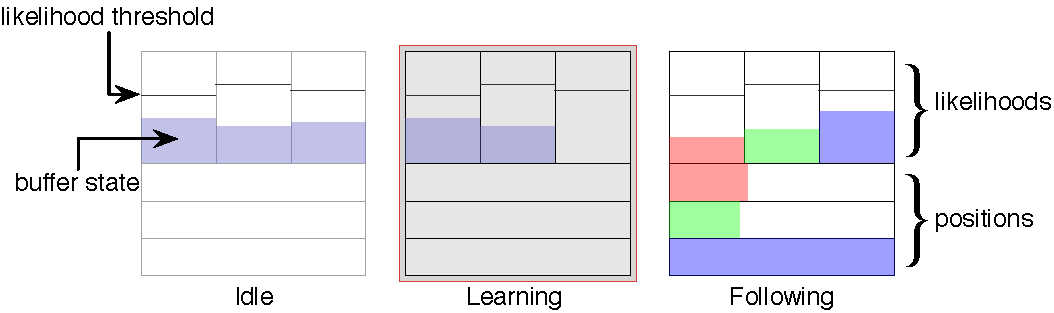
\includegraphics[width=0.95\columnwidth]{imgs/gesture-follower}
 \caption{The gesture follower appearance in its different phases.}
 \label{fig:gfgraph}
\end{figure}




%===============================
%:Appendix
\toplevel{Appendices}
\sublevel{Grammar definition}
\label{yacc}
\begin{verbatim}
//_______________________________________________
// relaxed simple INScore format specification
//_______________________________________________
start       : expr
            | start expr
            ;

//_______________________________________________
// expression of the script language
//_______________________________________________
expr        : message  ENDEXPR		
            | variabledecl ENDEXPR	
            | script            
            ;

//_______________________________________________
// javascript and lua support
//_______________________________________________
script      : LUASCRIPT            
            | JSCRIPT            
            ;
//_______________________________________________
// messages specification (extends osc spec.)
//_______________________________________________
message	    : address 
            | address params            
            | address watchparams		
            | address watchparams LEFTPAR messagelist RIGHTPAR
            | address watchparams script 
            ;

messagelist : message            		
            | messagelist COMMA message 
            ;

//_______________________________________________
// address specification (extends osc spec.)
address	    : oscaddress            	
            | urlprefix oscaddress		
            ;

oscaddress  : oscpath            		
            | oscaddress oscpath		
            ;

oscpath	     : PATHSEP identifier		
            | PATHSEP WATCH            	
            | PATHSEP VARSTART varname	
            ;

urlprefix   : hostname COLON UINT		
            | IPNUM COLON UINT            
            ;

hostname    : HOSTNAME            		
            | hostname POINT HOSTNAME	
            ;

identifier  : IDENTIFIER		
            | HOSTNAME            
            | REGEXP            
            ;

//_______________________________________________
// parameters definitions
// watchparams need a special case since messages are expected as argument
//_______________________________________________
watchparams : watchmethod		
            | watchmethod params 

params      : param            	
            | variable            
            | params variable	
            | params param		
            ;

watchmethod : WATCH            	
            ;

variable    : VARSTART varname
            | VARSTART LEFTPAR message RIGHTPAR
            ;

param       : number            
            | FLOAT            	
            | identifier		
            | QUOTEDSTRING		
            ;

//_______________________________________________
// variable declaration
variabledecl : varname EQUAL params	
            ;

varname	    : IDENTIFIER            
            | HOSTNAME            	
            ;

//_______________________________________________
// misc
number      : UINT            		
            | INT            		
            ;
\end{verbatim}


\sublevel{Lexical tokens}
\label{lex}
\begin{verbatim}
//_______________________________________________
// numbers
//_______________________________________________
INT       a signed integer
UINT      an unsigned integer
FLOAT     a floating point number

//_______________________________________________
// hosts addresses
//_______________________________________________
// allowed character set for host names (see RFC952 and RFC1123)
HOSTNAME       : [-a-zA-Z0-9]+ 
IPNUM          :  {DIGIT}+"."{DIGIT}+"."{DIGIT}+"."{DIGIT}+

//_______________________________________________
// OSC addresses
//_______________________________________________
// allowed characters for identifiers
IDENTIFIER     : [_a-zA-Z][_a-zA-Z0-9]*
REGEXP           see OSC doc for regular expressions
OSCADDRESS

//_______________________________________________
// strings
//_______________________________________________
STRING          : ("/"|(".""."?"/")*)([^ \t\\/?:*><|"';=]+"/"?)+"."[_a-zA-Z0-9]+
                  or quoted strings that can include any character
                  quotes could be single (') or double quotes (")

//_______________________________________________
// scripting
//_______________________________________________
JSCRIPT        : <?javascript any javascript code ?>
VARIABLE       : the name of a name

//_______________________________________________
// misc.
//_______________________________________________
POINT          : '.'
VARSTART       : '$'
COLON          : ':'
COMMA          : ','
LEFTPAR        : '('
RIGHTPAR       : ')'
EQUAL          : '='
ENDEXPR        : ';'
ENDSCRIPT      : "__END__"
EVAL           : "eval"

//_______________________________________________
// score expressions
//_______________________________________________
EXPRESSION    expr( a valid score expression )
              see 'Score expressions grammar'

//_______________________________________________
// math expressions
//_______________________________________________
ADD            : '+'
DIV            : '/'
EQ             : '=='
GREATER        : '>'
GREATEREQ      : '>='
LESS           : '<'
LESSEQ         : '<='
MINUS          : '-'
MODULO         : '%'
MULT           : '*'
NEG            : '!'
QUEST          : ' ? '
SUB            : '- '
MAX            : '@max' 
MIN            : '@min'

VARIABLEPOSTDEC : $VAR--
VARIABLEPOSTINC : $VAR++
VARIABLEPREDEC  : --$VAR
VARIABLEPREINC  : ++$VAR

\end{verbatim}




%===============================
%:Changes list
\toplevel{ Changes list}
\label{changes}


%===============================
%:    Differences to version 1.08  (version 1.12)
\sublevel{Differences to version 1.08}
\begin{itemize}
\item new \OSC{preserve} method at application level, provided to preserve previous behaviors. See section \fullref{applmgmt}.
\item default size of guido item is increased.
\item new \OSC{arrows} attribute for \OSC{line} objects. See section \fullref{arrows}.
\item incoming messages buffer size increased to 10.000
\item url support for inscore files (\OSC{load} message)

\item new common queries (\OSC{get} message) : \OSC{count} and \OSC{rcount} that give the enclosed objects count and recursive count. The messages are supported at scene and application level as well. See section \fullref{scenequery}.
\item new \OSC{memimg} object that capture the image of any object hierarchy including scenes. See section \fullref{imgscore}.
\item supports relative OSC addresses that are evaluated in the context of the target object 
  (i.e. a scene for drag and drop operations, arbitrary objects with the \OSC{eval} method). See section \fullref{scriptmsgs}.
\item new \OSC{eval} method that takes a message list as argument, provided as a context for relative addresses evaluation. See section \fullref{miscmsgs}.
\item new \OSC{httpd} object that implements an http server providing images of the scene to remote clients. See section \fullref{webobjects} and section \fullref{Httpd}.
\item new \OSC{websocket} object that implements a websocket server providing images of the scene to remote clients but also changes notifications. See section \fullref{webobjects}.

\item  Files objects can receive URL as path. See section \fullref{filebasedrsrc}.
\item new intermediate object for the URL (waiting for the data to be downloaded to create the real object)
\item new events associated to url based objects: success, error, cancel. See section \fullref{urlevents}.
\item  support for int values as parameters of the set method of rect shape and polygon objects
\item  the \OSC{clear} message addressed to a \OSC{gmnstream} object clears also the view. The change was not previously reflected until a new valid string was posted to the object.


\item bug in export item corrected : child scaling was not applied.
\item bug correction: for multiple exports, only the last one was done.
\item bug in extended address support corrected: extended address was ignored for messages dropped to a scene .
\item bug in window color corrected: black color was not correctly set due to an incorrect color 
  information returned by Qt.
\item bug with 'line' initialization corrected: wrong position and orientation with negative coordinates (was previously corrected but reintroduced), incorrect initialization in layers.

\end{itemize}

%===============================
%:    Differences to version 1.07
\sublevel{Differences to version 1.07}
\begin{itemize}
\item  new \OSC{\_\_END\_\_} marker supported to end a script parsing at arbitrary location  (see section \fullref{scriptstatement}).
\item  when displaying the mapping, the map dates are not printed any more by default (due to size and collisions).  The debug map parameter change from boolean to int value: 1 to activate the mapping display, 
2 to have also the dates displayed  (see section \fullref{debugnode}).
\item the signal node is available at any level of the hierarchy (as well as the sync node)
\item new \OSC{connect} and \OSC{disconnect} messages for the signal node to support signal connection to objects graphic attributes (see section \fullref{signalcnx}).
\item a slave can have several masters
\item no more side effects for synchronized objects (position change, scaling)
\end{itemize}

%===============================
%:    Differences to version 1.06
\sublevel{Differences to version 1.06}
\begin{itemize}
\item bug with 'line' initialization corrected: wrong position and orientation with negative coordinates.
\item new \OSC{plugins} static node at application level to provide a user path to look for pugins (see section \fullref{ITLplugins}).
\item explicit objects for musicxml scores (\OSC{musicxml} and \OSC{musicxmlf} types) (see section \fullref{symscore}).
\item new \OSC{faustdsp} object, charging libfaust as a plugin to compile faust DSP on-the-fly (see section \fullref{sigscore}).
\item exception catched when sending osc messages: was a potential crash, 
  e.g. in case of \OSC{get} message sent to a signal with a large buffer -> out of buffer memory
\item new javascript 'post' function for posting delayed messages  (see section \fullref{jsobj})
\item new \OSC{write} method supported by the 'log' window (see section \fullref{ITLlog})
\item variable addresses are evaluated in message based variables
\item supports relative rotations on x and y axis
\end{itemize}

%===============================
%:    Differences to version 1.05
\sublevel{Differences to version 1.05}
\begin{itemize}
\item \OSC{save} message can now take an optional list of attributes to be saved  (see section \fullref{common})
\item variables are now evaluated and expanded inside strings. Thus interaction variables can now be passed as argument of javascript functions.
\item corrects musicxml-version output
\item log window is put to front when the show menu is recalled
\item object aliases are removed when the object is deleted
\end{itemize}

%===============================
%:    Differences to version 1.03
\sublevel{Differences to version 1.03}
\begin{itemize}
\item incorrect error message for watch messages corrected
\item new javascript \OSC{readfile} function (see section \fullref{jsobj})
\item log window is now available from the application 'Tools' menu
\item new \OSC{brushStyle} attribute (see section \fullref{brush})
\item new \OSC{layer} object (see section \fullref{miscscore})
\item new \OSC{save} method specific to the log window: saves the window content to a file (see section \fullref{ITLlog})
\item new \OSC{event} method supported at object level for UI events simulation
\item new \OSC{del} watchable event: sent when deleting an object (see section \fullref{miscevents})
\item new \OSC{gmnstream} guido stream object (see section \fullref{symscore})
\end{itemize}

%===============================
%:    Differences to version 1.0
\sublevel{Differences to version 1.0}
\begin{itemize}
\item log window utility provided as a new static node at application level (\OSC{/ITL/log}) (see section \fullref{ITLlog}).
\item new \OSC{systemCount} read only attribute for Guido scores (see section \fullref{gmnpage})
\item IRCAM gesture follower support (see section \fullref{GF})
\item javascript engine is available at the static address /ITL/scene/javascript and can be activated using a 'run' method  (see section \fullref{jsobj})
\item new \OSC{export} event (see section \fullref{miscevents})
\item new \OSC{endPaint} event at scene level  (see section \fullref{miscevents})
\item new \OSC{windowOpacity} method at scene level (see section \fullref{scene})
\item bug correction: error messages not generated for dropped files (actually for the scene load method)
\item bug correction: possible infinite loop in QStretchTilerItem::paint method
\item bug correction: incorrect get alias output (all the aliases were dumped out in a single message)
\end{itemize}

%===============================
%:    Differences to version 0.98
\sublevel{Differences to version 0.98}
\begin{itemize}
\item bug correction in streching very small objects (due to approximations)
\item bug correction in \$sx and \$sy computation (xorigin and yorigin was not taken into account)
\item new 'ticks' message at application level for querying or setting the current count of time tasks (see section \fullref{applmgmt})
\item new 'time' message at application level for querying or setting the current time (see section \fullref{applmgmt})
\item new 'forward' message at application level for messages forwarding to remote hosts (see section \fullref{applmgmt})
\item new 'relative | absolute' synchronization mode (see section \fullref{syncmode})
\item 'rename' message not supported any more
\item a scene accepts multiple dropped files
\item significant extension and syntax changes in inscore script files (see Scripting documentation section \fullref{scripting})
\item fileWatcher methods renamed and simplified (see section \fullref{filewatch})
\item 'click' and 'select' messages are not supported any more.
\item new 'stats' virtual node at application level (address /ITL/stats), supports 'get' and 'reset' messages
  the node gives statistics about the incoming messages (see section \fullref{ITLdebug})
\item crash bug in signal creation corrected: a signal size created with an incorrect stream 
  (e.g. a string value) was 0 and no buffer was allocated.
\item extension of the time related events to duration: new 'durEnter' and 'durLeave' watchable events (see section \fullref{timeevents})
\item new 'absolutexy' message at scene level to switch to absolute coordinates (in pixels) (see section \fullref{scene})
\item new 'push' and 'pop' messages to store and restore current watched events and associated messages (see section \fullref{evtstate})
\item internal change: mappings are now implemented as a separable library strictly complying to the 
  mappings formalism.
\item new \%f format for the date variable to request a float value (instead a rational value) (see section \fullref{timevar}).
\item dates may be specified as rational strings (see section \fullref{time}).
\item interaction messages are not any more generated when the date can't be resolved.
\item new \OSC{rate} message at application level to control the time task rate (see section \fullref{ITL})
\item new \OSC{frameless} message at scene level to switch to frameless or normal window (see section \fullref{scene})
\end{itemize}

%===============================
%:    Differences to version 0.97
\sublevel{Differences to version 0.97}
\begin{itemize}
\item new \OSC{fastgraph} object for graphic signals fast rendering (see section \fullref{setsect})
\item \$date variable overflow catched
\item files dropped on application icon correctly opened when the application is not running
\item supports drag and drop of textual osc message strings
\item osc error stream normalized: the message address is 'error:' or 'warning:'
   followed by a single message string.
\item javascript and lua support: a single persistent context is created at application level and for each scene. 
(see section \fullref{scriptlang})
\end{itemize}

%===============================
%:    Differences to version 0.96
\sublevel{Differences to version 0.96}
\begin{itemize}
\item  objects position, date and watched events preserved through type change
\item  bug in quantified dates corrected (null denominator set to the quantified value)
\item  new 'alias' message providing arbitrary OSC addresses support
\item  bug in parser corrected: \verb+\+ escape only ' and " chars, otherwise it is literal
\item  guido score map makes use of the new guidolib extended mapping API for staff and system
\item  chords map correction (corrected by guido engine) 
\end{itemize}

%===============================
%:    Differences to version 0.95
\sublevel{Differences to version 0.95}
\begin{itemize}
\item switch to v8 javascript engine
\item lua not embedded by default
\end{itemize}

%===============================
%:    Differences to version 0.92
\sublevel{Differences to version 0.92}
\begin{itemize}
\item new 'mouse' 'show/hide' message supported at application level (see section \fullref{ITL})
\item graphic signal supports alpha messages at object level
\item javascript and lua embedded and supported in inscore scripts  (see section \fullref{scriptlang}).
\item bug correction in sync delete (introduced with version 0.90)
\end{itemize}

%===============================
%:    Differences to version 0.91
\sublevel{Differences to version 0.91}
\begin{itemize}
\item bug corrected: crash with messages addressed to a signal without argument
\item date and duration messages support one arg form using 1 as implicit denominator value 
  the one arg form accepts float values  (see section \fullref{time}).
\end{itemize}

%===============================
%:    Differences to version 0.90
\sublevel{Differences to version 0.90}
\begin{itemize}
\item bug in sync management corrected (introduced with the new sync parsing scheme)
\end{itemize}

%===============================
%:    Differences to version 0.82
\sublevel{Differences to version 0.82}
\begin{itemize}
\item at application level: osc debug is now 'on' by default
\item new scripting features (variables)  (see section \fullref{scriptvar}).
\item ITL file format change: \\
  - semicolon added at the end of each message \\
  - '//' comment not supported any more \\
  - '\%' comment char replaced by '!' \\
  - new variables scripting features \\
  - single quote support for strings \\
  - messages addressed to sync node must use the string format
\item new 'grid' object for automatic segmentation and mapping
\end{itemize}

%===============================
%:    Differences to version 0.81
\sublevel{Differences to version 0.81}
\begin{itemize}
\item new Faust plugins for signals processing
\item colors management change: all the color models (RGBA and HSBA) accept now
  float values that are interpreted in the common [-1,1] range. For the
  hue value, 0 always corresponds to 'red' whatever the scale used.
\item stretch adjustment for video objects (corrects gaps in sync h mode)
\item support for opening inscore files on the command line
\item system mapping correction
\item splash screen and about menu implemented by the viewer
\end{itemize}

%===============================
%:    Differences to version 0.80
\sublevel{Differences to version 0.80}
\begin{itemize}
\item behavior change with synchronization without stretch: now the system looks also in the
  slave map for a segment corresponding to the master date.
\item \OSC{\$date} variable change: the value is now (0,0) when no date is available and \OSC{\$date} is time shifted according to the object date.
\item \OSC{date} message change: the date 0 0 is ignored
\end{itemize}


%===============================
%:    Differences to version 0.79
\sublevel{Differences to version 0.79}
\begin{itemize}
\item corrects the map not saved by the \OSC{save} message issue
\item corrects \OSC{get map} output: 2D segments were not correctly converted to string
\end{itemize}

%===============================
%:    Differences to version 0.78
\sublevel{Differences to version 0.78}
\begin{itemize}
\item crash bug corrected for the 'save' message addressed to '/ITL'
\item message policy change: relaxed numeric parameters policy (float are accepted for int and int for float)
\item bug in \OSC{get watch} for time events corrected (incorrect reply)
\end{itemize}
Known issues:
\begin{itemize}
\item map not saved by the \OSC{save} message 
\end{itemize}

%===============================
%:    Differences to version 0.77
\sublevel{Differences to version 0.77}
\begin{itemize}
\item guido system map extended: supports flat map or subdivided map (see section \fullref{guidomap}).
\item new \OSC{shear} and \OSC{rotate} transformations messages (see section \fullref{transform}).
\item new \OSC{rename} message to change an object name (and thus its OSC address) (see section \fullref{common}).
\item relaxed bool parameter policy: objects accept float values for bool parameters 
\item automatic numbering of exports when destination file is not completely specified 
  i.e. no name, no extension. (see section \fullref{common}).
\item quantification introduced to \$date variable (see section \fullref{interactvar}).
\item \OSC{reset} message addressed to a scene clears the scene rootPath
\end{itemize}

%===============================
%:    Differences to version 0.76
\sublevel{Differences to version 0.76}
\begin{itemize}
\item  get \OSC{guido-version} and \OSC{musicxml-version} messages supported by the application (see section \fullref{ITL}).
\item  \OSC{save} message bug correction - introduced with version 0.70: only partial state of objects was saved
\item  \OSC{rootPath} message introduced at scene level (see section \fullref{scene}).
\item  scene name translation strategy change: only the explicit 'scene' name is 
  translated by the scene load message handler into the current scene name, 
  other names are left unchanged.
\item  bitmap copy adjustment in sync stretched mode is now only made for images
\end{itemize}


%===============================
%:    Differences to version 0.75
\sublevel{Differences to version 0.75}
\begin{itemize}
\item new \OSC{require} message supported by the \OSC{/ITL} node (see section \fullref{ITL}).
\item new event named \OSC{newElement} supported at scene level (see section \fullref{timeevents}).
\item new \OSC{name} and \OSC{address} variables (see section \fullref{interactvar}).
\item new system map computation making use of the new slices map provided by the guidolib version 1.42
\item INScore API: the \OSC{newMessage} method sets now the message src IP to localhost
  With the previous version and the lack of src IP, replies to queries or error 
  messages could be sent to undefined addresses (and mostly lost).
\item bug corrected with ellipse and rect : integer graphic size computation changed 
  to float (prevents objects disappearance with small width or height)
\item bug in scene export: left and right borders could be cut, depending  on the scene size
  corrected by rendering the QGraphicsView container instead the QGraphicsScene
\item crash bug with \$date:name corrected: crashed when there is no mapping named \OSC{name}.
\end{itemize}

%===============================
%:    Differences to version 0.74
\sublevel{Differences to version 0.74}
\begin{itemize}
\item new \OSC{map+} message  (see section \fullref{mapAddMsg}).
\item the \OSC{click} and \OSC{select} messages are deprecated (but still supported). They will be removed in a future version.
\end{itemize}

%===============================
%:    Differences to version 0.63
\sublevel{Differences to version 0.63}
\begin{itemize}
\item new \OSC{dpage} message accepted by \OSC{gmn} objects (see section \fullref{gmnpage}).
\item x and y variables: automatic range type detection (int | float)
\item set \OSC{txt} message: accepts polymorphic stream like parameters (see section \fullref{setsect}).
\item drag and drop files support in INScore viewer
\item interaction variables extension: \OSC{\$sx}, \OSC{\$sy} variables added to support scene coordinate space (see section \fullref{interactvar}).
\item automatic range mapping for \OSC{\$x}, \OSC{\$y} variables.
\item new \OSC{\$self} and \OSC{\$scene} variables in the address field (see section \fullref{oscvar}).
\item OSC identifiers characters set extended with '\_' and '-' (see section \fullref{genformat}).
\item support for multiple scenes: \OSC{new}, \OSC{del} and \OSC{foreground} messages (see section \fullref{scene}).
\item \OSC{load} message supported at scene level (see section \fullref{scene}).
\item \OSC{get watch} implemented.
\item \OSC{watch} message without argument to clear all the watched events (see section \fullref{interactvar}).
\item order of rendering and width, height update corrected (may lead to incorrect rendering)
\item bug with gmn score corrected: missing update for page, columns and rows changes.
\item package delivered with the Guido Engine version 1.41 that corrects minimum staves distance and incorrect mapping when optimum page fill is off.
\end{itemize}

%===============================
%:    Differences to version 0.60
\sublevel{Differences to version 0.60}
\begin{itemize}
\item new 'mousemove' event (see section \fullref{uievents}).
\item interaction messages accept variables (\$x, \$y, \$date...) (see section \fullref{interactvar}).
\item SVG code and files support (see section \fullref{setfile}).
\item set line message change: the \OSC{x y} form is deprecated, it is replaced by
  the following forms: \\
  \OSC{'xy' x y} (equivalent to the former form) 
  and \OSC{'wa' width angle}   
  (see section \fullref{setsect}).
\item new 'effect' message  (section \fullref{effectmsg}).
\item utf8 support on windows corrected
\item transparency support for stretched synchronized objects corrected
\item multiple application instances supported with dynamic udp port number allocation.
\item command line option with --port portnumber option to set the receive udp port number at startup.
\end{itemize}

%===============================
%:    Differences to version 0.55
\sublevel{Differences to version 0.55}
\begin{itemize}
\item new 'xorigin' and 'yorigin' messages (section \fullref{origin}).
\item new interaction messages set (section \fullref{interaction}).
\item alpha channel handled by images and video
\item bug correction in line creation corrected (false incorrect parameter returned)
\item bug correction in line 'get' message handling
\item memory leak correction (messages not deleted)
\end{itemize}

Known issues: 
\begin{itemize}
\item incorrect graphic rendering when 'sync a b' is changed to 'sync b a' in the same update loop
\item incorrect nested synchronization when master is horizontaly stretched,
\end{itemize}

%===============================
%:    Differences to version 0.53
\sublevel{Differences to version 0.53}
\begin{itemize}
\item ITL parser corrected to support regexp in message string (used by messages addressed to sync node)
\item format of mapping files and strings changed (section \fullref{mapMsg}).
\item format of sync messages extended to include map name (section \fullref{syncmsg}).
\item signal node: 'garbage' message removed
\item new 'reset' message for the scene (/ITL/scene) (section \fullref{scene}).
\item new 'version' message for the application (/ITL) (section \fullref{ITL}).
\item new 'reset' message for signals (section \fullref{ssignal}).
\item bug parsing messages without params corrected
\item slave segmentation used for synchronization
\item new H synchronization mode (preserves slave segmentation)
\item crash bug corrected for load message and missing ITL files
\end{itemize}

%===============================
%:    Differences to version 0.50
\sublevel{Differences to version 0.50}
\begin{itemize}
\item Graphic signal thickness is now symmetrically drawn around y position.
\item ITL file format supports regular expressions in OSC addresses.
\item IP of a message sender is now used for the reply or for error reporting.
\item new \OSC{line} object (section \fullref{setsect}).
\item new \OSC{penStyle} message for vectorial graphics (section \fullref{specificMsg}).
\item new color messages \OSC{red, green, blue, alpha, dcolor, dred, dgreen, dblue} (section \fullref{common} and  \fullref{relpos}).
\item color values for objects are bounded to [0,255]
\item \OSC{get map} message behaves according to new map message (section \fullref{getsect}).
\item \OSC{get width} and  \OSC{get height} is now supported by all objects (section \fullref{getsect}).
\item  bug in signal projection corrected (index 0 rejected)
\item  bug in signals default value delivery corrected
\item  new \OSC{pageCount} message for guido scores
\item  debug nodes modified state propagated to parent node (corrects the debug informations graphic update issue)
\item rational values catch null denominator (to prevents divide by zero exceptions).

\end{itemize}

%===============================
%:    Differences to version 0.42
\sublevel{Differences to version 0.42}

\begin{itemize}
\item \OSC{identifier} specification change (section \fullref{genformat}).
\item new application \OSC{hello} and  \OSC{defaultShow} messages (section \fullref{ITL}).
\item new \OSC{load} and \OSC{save} messages  (sections \fullref{ITL} and  \fullref{common}).
\item \OSC{click} and \OSC{select} messages:
\begin{itemize}
\item \OSC{rightbottom} and \OSC{leftbottom} modes renamed to \OSC{bottomright} and \OSC{bottomleft}
\item new \OSC{center} mode for the \OSC{click} message
\item query mode sent back with the reply both for \OSC{click} and  \OSC{select} messages
\end{itemize}
\item new \OSC{file}, \OSC{html} and  \OSC{htmlf} types for the \OSC{set} message (section \fullref{setsect}).
\item \OSC{get} syntax change for the \OSC{scene}.
\item \OSC{fileWatcher} messages completely redesigned.
\item mappings can be identified by names (section \fullref{mapMsg}).
\item rect, ellipse, curve, line and polygon object support graphic to relative-time mapping
\item new synchronization modes for Guido scores: voice1, voice2, ... , staff1, staff2, ... , system, page.
\item Guido mapping manages repeat bars.
\item Graphic signals messages design (section \fullref{gsignal}).
\end{itemize}



\printindex

\end{document}
